%%%%%%%%%%%%%%%%%%%%%%%%%%%%%%%%%%%%%%%%%%%%%%%%%%%%%%%%%%%%%%%%%%%%%%%%%%%%%%%%
%% INITIAL ARL DOCUMENT BOILERPLATE

\documentclass[12pt]{arlticle}
\usepackage{pdflscape}
\usepackage{coseoul}
\usepackage{notoccite}% PREVENTS CITES IN CAPTIONS FROM MISNUMBERING YOUR REFERENCES
% THANKS TO ADAM SOKOLOW FOR THESE CONVENIENT USES OF totpages AND changepage PACKAGES
\usepackage{totpages}% FOR ITEM 18 OF THE SF298
\usepackage{changepage}% TO MAKE SURE CERTAIN THINGS START ON ODD PAGE #
% MACRO TO GO TO ODD PAGE, INSERTING "INTENTIONALLY LEFT BLANK" IF
% NEEDED
\newcommand\gotooddpage{\clearpage%
  \checkoddpage\ifoddpage\else\blankpage\fi\clearpage}
% MACRO TO FINISH ON EVEN PAGE, INSERTING "INTENTIONALLY LEFT BLANK" IF NEEDED
\newcommand\finishonevenpage{%
  \clearpage\checkoddpage\ifoddpage\else\blankpage\fi}
% ARL FOOTNOTE STYLE:
\usepackage[symbol,perpage]{footmisc}
%%%%%
% CHECK WITH ORGANIZATION TO SEE IF WHAT FOLLOWS IS LATEST MANDATORY DISTRIBUTION LIST
  \def\MandatoryDL{ARL-07-27-16(Unlimited).dls}% MANDATORY DISTRIBUTION LIST FILE
  \def\LocalMandatoryDL{blank.dls}% USED FOR DIRECTORATE LEVEL MANDATORY DISTRIBUTIONS
  \def\UserDL{user.dls}%      USER DISTRIBUTION LIST FILE
  \addtolength{\cftfignumwidth}{0.0ex}%  EXTEND WIDTH OF LOF LABEL IF USING
%                                        APPENDIX FIGURES .OR. > 99 FIGURES
  \addtolength{\cfttabnumwidth}{0.0ex}%  EXTEND WIDTH OF LOT LABEL IF USING
%                                        APPENDIX TABLES .OR. > 99 TABLES
%% IN ADDITION TO THE DEFAULT (COMPUTER-MODERN) MATH FONT, THE FOLLOWING
%% ALTERNATIVES ARE APPROVED FOR USE IN ARL REPORTS (OPTIONALLY CHOOSE ONE LINE)
%  \usepackage{eulervm,eufrak}
%  \usepackage{newtxmath}
%  \usepackage{mathptmx}
%%
%\nosectspace% THE DEFAULT, TURNS OFF \spaceout{} FOR SPREADING OUT SECTION HEAD TEXT
\sectspace% MAY NEED TO TURN THIS SETTING OFF IF YOU HAVE STUFF OTHER THAN 
%           TEXT, \color, OR \label IN YOUR SECTION TITLES

\pagenumbering{roman}


% Created 2017-01-08 Sun 23:39
% Intended LaTeX compiler: pdflatex
% If desired, can use the following command to put a
% "DRAFT" stamp on each page; Can also use optional argument for
% page classification markings, as in \PageStamp[UNCLASSIFIED].  Can
% turn off with \StopPageStamp.  See arlticle documentation for 
% further details.
% One can make the page stamp in color with, for example, 
%   \PageStamp[\textcolor{red}{EYES ONLY}]
%
% Default PageStamp is "DRAFT".  Can be used for class. markings
%\def\PageStampColor{red}% THIS LINE IS ONLY NEEDED TO CHANGE THE PAGE STAMP COLOR
%\PageStamp[Draft (\today)]%  <---COMMENT THIS LINE IF NO PAGE STAMP DESIRED

% COVER & TITLE PAGE INPUTS SPECIFIED IN THE FOLLOWING COMMANDS:
%\arlzipcode	{}%		For use, if other than 21005-5066, i.e., 5069
\arlrptno  {ARL-TN-0000}%		Uncomment and use, when needed
\pubdate   {September 2017}%	Uncomment and use, when needed
\arltitle  {GPU-Accelerated Symmetry Transform for Object Saliency}
\allauthors{Jason Owens}
\authorsA  {Jason Owens}
\organizationA	{Vehicle Technology Directorate, ARL}
%% NOTE THAT FOR CONTRACT REPORTS, THE ADDRESS IS INCLUDED IN \organizationA, etc.,
%% AS IN THE FOLLOWING LINE
% \organizationA{SURVICE Engineering Company\\4695 Millenium Dr.\\Belcamp, MD 21017-7722}
%\authorsB      {J. Vince Pulido}% Uncomment and use, if needed
%\organizationB {Dept. of Systems Engineering, University of Virginia}%		Uncomment and use, 
\distcodes[RDRL-VTA]{A}{}{}    % DISTRIBUTION STATEMENT A
%\distcodes[RDRL-WMP-C]{C}{3}{X} %	FOR DISTRIBUTION C3, WITH EXPORT CONTROL
%\UnderContract{W91CRB-09-D-0027}% FOR CONTRACT REPORTS, ARL-CR SERIES
%\FOUOPageStamp                  % FOR FOUO DOCUMENTS
%\FOIAexemptions{3}              % FOR ADDING FOIA EXEMPTIONS
%\AddDistributionReason{4}       % FOR ADDING REASON TO DISTRIBUTION STATEMENT 
%\AddDistributionReason{X}       % FOR ADDING EXPORT CONTROLLED TO DISTRIBUTION STATEMENT

\usepackage{graphicx}
\usepackage{savesym} \savesymbol{iint} \savesymbol{iiint} \usepackage{amsmath}  \usepackage{amssymb} 
\usepackage{color} 
\restoresymbol{T}{iint} \restoresymbol{T}{iiint} 
\usepackage{xifthen}
\usepackage{mathtools}
\usepackage{flushend}
\usepackage{marginnote}
\usepackage{setspace}
\usepackage[utf8]{inputenc}
\usepackage{tabularx}
\usepackage[hidelinks]{hyperref}
\usepackage{booktabs}
\usepackage{xfrac}
\usepackage{xparse}
\usepackage{threeparttable}
\usepackage[acronym,shortcuts]{glossaries}
\usepackage{needspace}
\usepackage{pifont}
\newcommand{\cmark}{\ding{51}}%
\newcommand{\xmark}{\ding{55}}%
%\usepackage{acro}
%\acsetup{first-style=short}
\usepackage{listings}
\usepackage{xcolor,colortbl}
\usepackage{rotating}
\usepackage{adjustbox}
\usepackage{algorithm}
\usepackage{algpseudocode}


%% Adjust captions to meet ARL standards
\usepackage{subcaption}
\captionsetup[figure]{labelfont=bf,textfont=bf,size=footnotesize,labelsep=space}
\captionsetup[subfigure]{labelfont=bf,textfont=bf,size=footnotesize,labelsep=space}
\captionsetup[table]{labelfont=bf,textfont=bf,size=footnotesize,labelsep=space}
\usepackage{ARLboxhandler}

%% Make tables smaller
\newcommand*{\smalltables}{\let\Tabular\tabular
\def\tabular{\sffamily\fontsize{7.000000}{8.400000}\selectfont\Tabular}
\definecolor{blue}{rgb}{0.316186,0.433203,0.916155}
\definecolor{lightblue}{rgb}{0.716186,0.833203,0.916155}}
\newcommand*{\restoretables}{\let\tabular\Tabular}

%%%%%%%%%%%%%%%%%%%%%%%%%%%%%%%%%%%%%%%%%%%%%%%%%%%%%%%%%%%%%%%%%%%%%%%%%%%%%%%%
%% support creating braces INSTEAD of parens when already inside parens
\newcommand*{\pac}[2][]{\ifglsused{#2}{\acs[#1]{#2}}{%
 \glsunset{#2}%
 \acl[#1]{#2} [\acs[#1]{#2}]}}

\newcommand{\ra}[1]{\renewcommand{\arraystretch}{#1}}
\ra{1.3}

%% COMMENT COMMANDS
\newcommand{\comment}[3]{\marginpar{\raggedright\setstretch{0.5}\textcolor{#1}{\scriptsize #2}}\textcolor{gray}{#3}} 
\newcommand{\hmmm}[2][]{\comment{orange}{#1}{#2}}
\newcommand{\jlo}[2][]{\comment{blue}{#1}{#2}}
\newcommand{\pro}[2][]{\comment{red}{#1}{#2}}
\newcommand{\jvp}[2][]{\comment{olive}{#1}{#2}}

%% FORMATTING

% ARL-compliant figure refs
\newcommand{\arlfig}[1]{Fig.~\ref{#1}}
\newcommand{\Arlfig}[1]{Figure~\ref{#1}}
\newcommand{\ie}{i.e.,~}
\newcommand{\eg}{e.g.,~}

%% MATH COMMANDS
\newcommand{\norm}[1]{\ensuremath{\left\lVert #1 \right\rVert}}
\renewcommand{\vec}[1]{\ensuremath{\mathbf{#1}}}
\newcommand{\neigh}[1]{\ensuremath{\mathcal{N}_{\vec{#1}}}}
\newcommand{\real}[1]{\ensuremath{\ifthenelse{\isempty{#1}}{\mathbb{R}}{\mathbb{R}^{#1}}}}
\newcommand{\Func}[1]{\ensuremath{\textbf{#1}}}
\renewcommand{\topfraction}{0.9}	% max fraction of floats at top
\renewcommand{\bottomfraction}{0.8}	% max fraction of floats at bottom
\newcommand{\vimg}{\ensuremath{\mathcal{I}}} 
\newcommand{\vrng}{\ensuremath{\mathcal{R}}} 
\newcommand{\vpcl}{\ensuremath{\mathcal{P}}}
\newcommand{\model}{\ensuremath{\mathcal{M}}}
\newcommand{\segments}{\ensuremath{\mathcal{S}}}
\newcommand{\vmask}{\ensuremath{\mathcal{V}}}
\newcommand{\true}{\ensuremath{\textbf{true}}}
\newcommand{\false}{\ensuremath{\textbf{false}}}
\newcommand{\normal}[1]{\ensuremath{\mathbf{\hat{#1}}}}
\newcommand{\normali}{\ensuremath{\normal{n}_i}}
\newcommand{\normalj}{\ensuremath{\normal{n}_j}}
\newcommand{\lseg}{\ensuremath{\vec{x}^j_i}}
\newcommand{\Rji}{\ensuremath{\prescript{i}{}{R_j}}}
\newcommand{\tji}{\ensuremath{\prescript{i}{}{\vec{t}_j}}}

\newcommand{\snode}{\ensuremath{\mathbb{S}}}
\newcommand{\lnode}{\ensuremath{\mathbb{L}}}
\newcommand{\pnode}{\ensuremath{\mathbb{P}}}
\newcommand{\sval}[1]{\ensuremath{\ifthenelse{\isempty{#1}}{\vec{x}^\snode}{\vec{x}_{#1}^\snode}}}
\newcommand{\lval}[1]{\ensuremath{\ifthenelse{\isempty{#1}}{\vec{x}^\lnode}{\vec{x}_{#1}^\lnode}}}
\newcommand{\pval}[1]{\ensuremath{\ifthenelse{\isempty{#1}}{\vec{x}^\pnode}{\vec{x}_{#1}^\pnode}}}
%\newcommand{\lval}[1]{\ensuremath{\vec{x}^\lnode}}
%\newcommand{\pval}[1]{\ensuremath{\vec{x}^\pnode}}
\newcommand{\typeof}[1]{\ensuremath{\mathrm{type}(#1)}}
\newcommand{\nodea}[1]{\ensuremath{\vec{x}_{#1}^\alpha}}
\newcommand{\nodeb}[1]{\ensuremath{\vec{x}_{#1}^\beta}}
\newcommand{\emean}[1]{\ensuremath{\vec{\mu}_{#1}}}
\newcommand{\proj}{\ensuremath{\pi}}
\newcommand{\pt}[1]{\ensuremath{\vec{p}_{#1}}}

\newcommand{\myparagraph}[1]{\textbf{\emph{#1}}.}

\renewcommand\[{\begin{equation}}
\renewcommand\]{\end{equation}}

%% environment for nice latex tables
%\newenvironment{asdtablewrap}[2]{%
%\newcommand{\hr}{\hline\addlinespace[0.1em]}
%\setlength{\tablecolsep}{12pt}}{}

% \thanks[*]{These authors have contributed equally to the content of this paper.}
%%%%%%%%%%%%%%%%%%%%%%%%%%%%%%%%%%%%%%%%%%%%%%%%%%
%% Commands for GAST
\newcommand{\Image}{\ensuremath{\mathcal{I}}}
\newcommand{\imgdom}{\ensuremath{\Omega}}
\newcommand{\integer}[1]{\ensuremath{\ifthenelse{\isempty{#1}}{\mathbb{Z}}{\mathbb{Z}^{#1}}}}
\newcommand{\var}[1]{{\ttfamily #1}}
\newcommand{\cmax}{C_{\max}}
\newcommand{\thetamax}{\theta_{\max}}
\newcommand{\pmin}{p_{\min}}
\newcommand{\pmax}{p_{\max}}
\newcommand{\T}{\ensuremath{^{\mkern1.5mu\mathsf{T}}}}
\newcommand{\atantwo}{\ensuremath{\operatorname{atan2}}}
\newcommand{\sym}{\ensuremath{M_\sigma(p)}}

\hyphenation{crystallography}

\lstdefinestyle{cuda}{
  language=C++,
  basicstyle=\scriptsize\ttfamily,
  keywordstyle=\bfseries\color{green!40!black},
  commentstyle=\itshape\color{purple!40!black},
  emph={__global__,blockIdx,blockDim,threadIdx,make_int2,int2,float2},
  emphstyle=\color{red!60!black},}

%%%%%%%%%%%%%%%%%%%%%%%%%%%%%%%%%%%%%%%%%%%%%%%%%%%%%%%%%%%%%%%%%%%%%%%%%%%%%%%%
%% Collect acronyms here!

\newacronym{2d}{2-D}{2-dimensional}
\newacronym{3d}{3-D}{3-dimensional}
\newacronym{cnn}{CNN}{convolutional neural network}
\newacronym{col}{COL}{continuous object learner}
\newacronym{dcf}{DCF}{discriminative correlation filter}
\newacronym{dft}{DFT}{discrete Fourier transform}
\newacronym{dnn}{DNN}{deep neural network}
\newacronym{dso}{DSO}{Direct Sparse Odometry}
\newacronym{dvo}{DVO}{Dense Visual Odometry}
\newacronym{cpu}{CPU}{central processing unit}
\newacronym{gpu}{GPU}{graphics processing unit}
\newacronym{icp}{ICP}{iterative closest point}
\newacronym{imu}{IMU}{inertial measurement unit}
\newacronym{ir}{IR}{infrared}
\newacronym{kcf}{KCF}{Kernelized Correlation Filter}
\newacronym{lstm}{LSTM}{long-short-term memory}
\newacronym{mdnet}{MDNet}{multidomain network}
\newacronym{mht}{MHT}{multiple hypothesis tracking}
\newacronym{mot}{MOT}{multiobject tracking challenge}
\newacronym{nl-lmp}{NL-LMP}{node labeling lifted multicut problem}
\newacronym{pcl}{PCL}{Point Cloud Library}
\newacronym{rnn}{RNN}{recurrent neural network}
\newacronym{sdf}{SDF}{signed distance function}
\newacronym{slam}{SLAM}{simultaneous localization and mapping}
\newacronym{svo}{SVO}{semi-direct visual odometry}
\newacronym{tsdf}{TSDF}{truncated signed distance function}
\newacronym{vo}{VO}{visual odometry}
\newacronym{cvpr}{CVPR}{Computer Vision and Pattern Recognition}
\newacronym{hog}{HOG}{histogram of oriented gradients}
\newacronym{rgb}{RGB}{red, green, blue}
\newacronym{rgbd}{RGB-D}{red, green, blue and depth}
\newacronym{lidar}{LIDAR}{light detection and ranging}
\newacronym{orb}{ORB}{oriented FAST and rotated BRIEF}
\newacronym{sift}{SIFT}{scale-invariant feature transform}
\newacronym{ros}{ROS}{Robot Operating System}
\newacronym{simd}{SIMD}{single-instruction multiple-data}
\newacronym{vga}{VGA}{Video Graphics Array}

\makeglossaries

%% how to use the acronyms:
% \gls{...} for an acronym
% \glspl{...} for a pluralized acronym
% \pac{...} for an acronym in a parenthetical

\begin{document}
\ARLcover{}
\arltitlepage

%% OPTION I: CREATE YOUR OWN SF298 in LaTeX:
\begin{createSFtwoNINEeight}
% SFitemONE AUTOMATICALLY FILLED IN (\pubdate)
% SFitemTWO AUTOMATICALLY FILLED IN (Final)
  \SFitemTHREE{November 2016-September 2017}
% SFitemFOUR AUTO-FILLED WITH \arltitle DATA
% SFitemFIVEa AUTO-FILLED WITH \UnderContract DATA
% \SFitemFIVEb{[Grant Number here]}
% \SFitemFIVEc{[PE Number here]}
  \SFitemFIVEd{APPLE}
% \SFitemFIVEe{[Task No. here]}
% \SFitemFIVEf{[WU Number here]}
% SFitemSIX{} AUTO-FILLED WITH \allauthors DATA
  \SFitemSEVEN{US Army Research Laboratory\\ATTN: 
               RDRL-VTA\\Aberdeen Proving Ground, MD 21005-5066}
% SFitemEIGHT AUTOMATICALLY FILLED IN (\arlrptno)
% \SFitemNINE{[Sponsor here]}
% \SFitemTEN{[Sponsor Acronym]}
% \SFitemELEVEN{[Sponsor Rpt. No.]}
% SFitemTWELVE AUTOMATICALLY FILLED IN WITH \distcodes DATA
  \SFitemTHIRTEEN{Primary author's email:
    $<$jason.l.owens.civ$@$mail.mil$>$.}

  \SFitemFOURTEEN{ This technical note describes a method to compute a symmetry transform in 2 dimensional images, based on matching image gradients around a center reference point. The method is particularly amenable to parallel processing, and we describe an implementation that runs on graphics processing units for significantly reduced execution time for VGA sized images. The symmetry transform has potential for use in finding salient regions containing object, and also may be applicable to stable object keypoints for recognition. }

  \SFitemFIFTEEN{\footnotesize symmetry, parallel processing, object recognition, perception, intelligent systems }
% \SFitemSIXTEENa defaults to UNCLASSIFIED
% \SFitemSIXTEENb defaults to UNCLASSIFIED
% \SFitemSIXTEENc defaults to UNCLASSIFIED
% SFitemSEVENTEEN AUTOMATICALLY FILLED IN WITH "SAR" or "UU"
% ITEM 18 CAN BE AUTOMATICALLY OBTAINED WITH \ref{TotPages}, USING THE totpages PACKAGE
  \SFitemEIGHTEEN{\ref{TotPages}}%	= FRONT MATTER PP. + REPORT PP. + 2
  \SFitemNINETEENa{Jason Owens}
  \SFitemNINETEENb{410-278-7023}
\end{createSFtwoNINEeight}
\tableofcontents%		p. iii
\listoffigures%			Comment out, if not needed
%\listoftables*%			Comment out, if not needed
\glsresetall

\gotooddpage
\pagenumbering{arabic}%		p. 1

%%%%%%%%%%%%%%%%%%%%%%%%%%%%%%%%%%%%%%%%%%%%%%%%%%%%%%%%%%%%%%%%%%%%%%%%%%%%%%%%
%% Start Document Content
\section{Introduction}
\label{sec:intro}
Finding salient object candidates in arbitrary natural images is a problem in computer vision and robotic perception that has yet to be solved. There are many ways this challenge is currently approached: (1) scan the entire image, at multiple scales, with some kind of object recognition algorithm, generating a heat map indicating the score or probability of a known, detected object (i.e. sliding window); (2) propose a smaller set of likely object regions based on some engineered or learned features of the image (e.g. edge boxes, geodesic object proposals, objectness); (3) compute a segmentation of the image to propose object-like regions; or (4) learn a saliency function to predict regions of the image that may contain objects.

In recent years and in combination with advanced deep learning systems for object recognition tasks, the use of some kind of object proposal algorithm has become a de facto standard. Since object proposal algorithms produce a significantly smaller number of image regions to test than almost any other mechanism (\eg sliding window), they are used to speed up existing detection algorithms by reducing the number of times an object model must be checked. The main idea for many proposal algorithms is to either engineer or train a detector for what has been called the "objectness" of a region, \ie how well that region reflects aspects of an image of an object. Object aspects often include such properties as closed contours, convexity, and compactness \cite{koffka_principles_1935}. In the image domain, the contours can often be reflected in the edges derived from the image gradient.

However, processing image contours without any additional information (\eg learning an object contour prior) often yields undesirable results, with many proposals that do not represent an object. When we discuss objectness, we usually care about whole physical objects we can pick up (box of cereal, phone, pencil, flashlight, coffee mug) and not the aspects of an object's appearance that may also provide strong gradient edge responses, e.g. logos or pictures on a cereal box.

In 1995, Reisfeld et al. proposed the use of a symmetry transform operator\cite{reisfeld_robust_1992} in the image domain for use as an attentional operator. Since symmetry is considered a strong indicator of an object with shape\cite{dickinson_symmetry_2013}, it's reasonable to conclude that regions exhibiting strong symmetry are likely to contain objects of interest.

Reisfeld showed that by extracting contours from the symmetry magnitude and selecting local maxima, it was possible to compute attention keypoints that indicated important features of the image. For example, \arlfig{fig:salient} shows an example from \cite{reisfeld_context_1995} where selecting the maximum output of the radial symmetry transform produces keypoints for the face of Nixon, the forehead of Elvis, as well as several interesting points on the flags.

\begin{figure}[htbp]
\centering
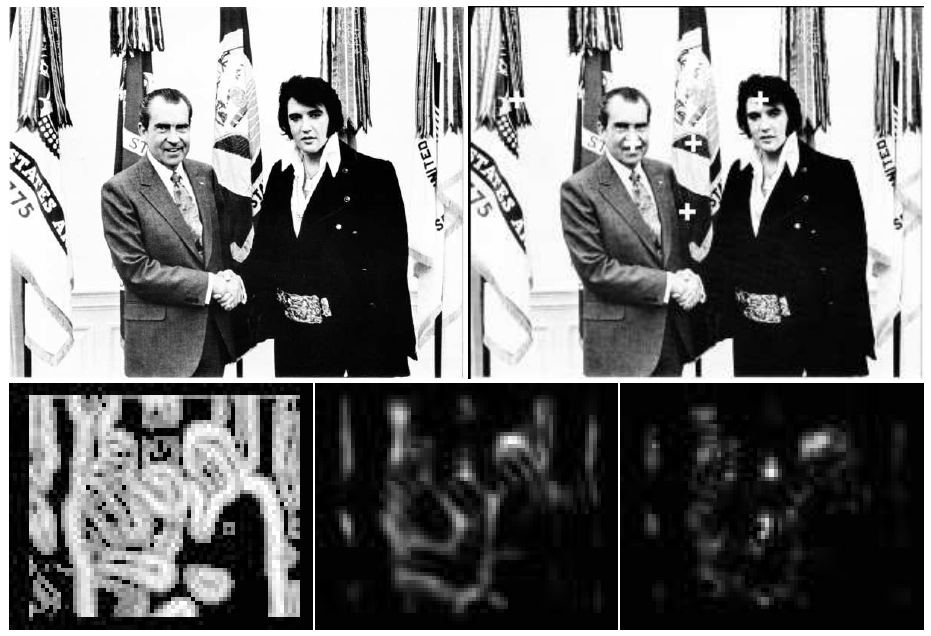
\includegraphics[width=0.5\linewidth]{Introduction/elvis.png}
\caption{\label{fig:salient}
Salient keypoint extraction using symmetry magnitude, reproduced from \citenum{reisfeld_context_1995}}
\end{figure}

Kootstra et al. have focused on the use of Gestalt features specifically for attention and segmentation of known objects\cite{kootstra_using_2010,kootstra_gestalt_2011}, exploiting and expanding on the concepts put forth by Reisfeld\footnote{Kootstra's work, in fact, was the inspiration for this investigation into implementing and parallelizing the symmetry transform for use in object saliency and proposal.}. They found that while the symmetry informed the saliency and object proposal detection, their strong assumption that objects rest on (and protrude from) dominant planes proved the most useful at predicting object presence. 

Potapova et al.\cite{potapova_local_2012} eschews the \gls{2d} appearance-based symmetry and constructs a \gls{3d} approach using depth maps derived from stereo or \gls{rgbd} sensors, and compute symmetry by matching surface normal directions instead of gradient directions. The authors show this yields better objectness results than the appearance-based approach of Kootstra.

\subsection{Problem}
\label{sec:problem}

In general, we want to solve the ill-defined problem of finding regions in the image that contain objects or object parts. Objects are things in the world that are compact and have reasonably well-defined boundaries, and therefore will often be visible almostly completely within an image frame. In contrast, ``stuff'' in the world is less well-bounded, and perhaps more amorphous and spread out; \eg walls, carpet, and even desktops or counters in indoor environments. For an autonomous mobile agent, which needs to adapt and learn online in new environments, the ability to detect potential objects is necessary for both recognition and continuous learning. This larger task of continuous online learning is outside the scope of this note, but serves to define the context for an object saliency measure.

In the theory of Gestalt perception, the whole is considered more than the sum of its parts\cite{jakel_overview_2016}. Some of the phenomena that trigger this process include symmetry, continuity, and connectedness. In the context of this work, we are focusing on contours and accumulating the nature of their symmetry over the content of the image. The goal is to find regions associated with symmetric contours, and thereby derive some measure of the salience of the region using the following observation: objects, by the nature of their shape and ``well-boundedness,'' exhibit symmetry in their countours and boundaries. The rest of this note describes one method, and a specific implementation of it, for computing a transform that reflects the amount of symmetry surrounding a point, based on matching the direction of the gradients in the neighborhood of the point. 

\subsection{Contributions}
\label{sec:contributions}

In the following sections, we document our work implementing the symmetry algorithm directly from Reisfeld's mathematical formulation as an NVIDIA CUDA kernel for \gls{gpu} acceleration. We make the following contributions: a brief analysis of the computational implications of the algorithm, leading to the parallel nature of the problem; algorithm and source listing for the parallel kernel; and a brief discussion of the GPU performance and the output of a simple salient point detector. 

\section{Mathematical Approach}
\label{sec:mathematical}

Reisfeld's symmetry transform uses the gradient image to compute symmetry magnitude and direction for every pixel in the image. Given the magnitude image, one can then use non-maximum suppression to select local maxima as salient points in order to direction attentional processing. For convenience, we restate Reisfeld's mathematical formulation to provide background for the computational approach discussed in the next section. 

Let \(\Image\,:\,\imgdom \to [0,1]\) be a grayscale image with domain \(\imgdom \subset \integer{2}\). Then \(p_k \in \imgdom\) represents some pixel coordinate in the image, and \(\nabla(p_k) = \left(\frac{\partial}{\partial x}\Image(p_k), \frac{\partial}{\partial y}\Image(p_k) \right)\) is the gradient at that coordinate. Reisfeld then computes a 2D polar coordinate for each pixel, \((r_k,\theta_k)\), where \(r_k = \log(1 + \norm{\nabla(p_k)})\), and \(\theta_k = \atantwo(\frac{\partial}{\partial y}\Image(p_k),\frac{\partial}{\partial x}\Image(p_k))\). Let \(l_{ij}\) be the line passing through two points \(p_i\) and \(p_j\), and let \(\alpha_{ij}\) be the angle \(l_{ij}\) makes with the horizontal (\(x\)) axis. For any pixel \(p_k\), define the set \(\Gamma(p_k) = \{ (i,j) \mid \frac{p_i + p_j}{2} = p_k \}\), i.e. the set of pixel index pairs such that \(p_k\) resides on the center of the separating line \(l\). A distance, \(D_\sigma(i,j)\), and phase, \(P(i,j)\) function are used to determine the contribution \(C(i,j)\) for each point pair in \(\Gamma(p_k)\), defined as follows:

\begin{align}
D_\sigma(i,j) &= \frac{1}{\sqrt{2\pi}\sigma}e^{-\frac{\norm{p_i - p_j}}{2\sigma}} \label{eq:dist} \\
P(i,j)        &= \left(1 - \cos(\theta_i + \theta_j - 2\alpha_{ij})\right)\left(1 - \cos(\theta_i - \theta_j)\right) \label{eq:phase}\\
C(i,j)        &= D_\sigma(i,j)P(i,j)r_i r_j \label{eq:cont}
\end{align}

Finally, the \emph{symmetry magnitude} for a point \(p\) is defined as:
\[ \sym = \sum_{(i,j) \in \Gamma(p)} C(i,j) \] which simply sums the weighted contributions over the entire ``symmetric pixel'' neighborhood of \(p\) (producing an averaged value). A direction contribution function for each pixel, \(\psi(i,j)\), used to compute the \emph{symmetry direction}, \(\operatorname{\phi}(p)\) for \(p\), is defined as follows:

\begin{align}
\psi(i,j) &= \frac{\theta_i + \theta_j}{2} \\
\phi(p)   &= \psi(i^*,j^*)\quad\mathrm{where}\quad(i^*,j^*) = \operatorname*{argmax}_{(i,j) \in \Gamma(p)} C(i,j)
\end{align} 

We can then define the overall output of the symmetry transform as:
\[S_\sigma(p) = \{\sym, \phi(p)\}.\] Please see \arlfig{fig:pixel-contr} for an illustration indicating the values involved in the transform.

\Needspace{0.3\textheight}
\begin{figure}[ht]
\centering
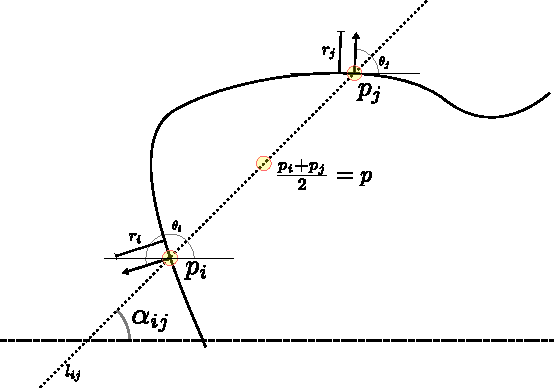
\includegraphics[width=0.6\linewidth]{figures/pixel_contributions.pdf}
\caption{\label{fig:pixel-contr}
Illustration of the geometry and quantities involved in computing pixel pair contributions for the image gradient symmetry around point \(p\)}
\end{figure}

Note that in the original paper, Reisfeld justifies using the logarithm of the gradient magnitude in order to reduce the contribution of stronger gradients and makes the correlation measure (\(C(i,j)\)) less sensitive to stronger edges. Also note that the 2D Gaussian function used in the distance function is circular; Reisfeld points out that this can be modified to emphasize elliptical features. In addition, he defines a modified symmetry magnitude he calls \emph{radial symmetry} that emphasizes symmetries that are perpendicular to the primary symmetry direction (i.e. \(\phi(p)\):

\[ RS_\sigma(p) = \sum_{(i,j) \in \Gamma(p)} C(i,j) \sin^2 \left(\psi(i,j) - \phi(i,j)\right). \] 

An important aspect of this function is to note that the \(\sym\) value must already be computed (and \(C(i,j)\) computed twice, or otherwise cached), by virtue of the use of \(\phi(i,j)\), since it is a function of the entire neighborhood \(\Gamma(p)\).

\section{Computational Approach}
\label{sec:computational}
From the mathematical definition of the symmetry transform, we can see that there are no mutual data dependencies between pixels given the gradient image; in other words, the problem is embarrassingly parallel. Each pixel \emph{does} depend on a neighborhood (defined both by equation \ref{eq:dist} and \(\Gamma(\cdot)\)), but \(\sym\) does not need values computed by any other neighboring pixel. We can therefore compute the symmetry transform for each pixel independently, which suggests that an adaptation of the algorithm for \gls{gpu} computation should be relatively straightforward. 

In this section, we present the basic sequential algorithm (with no optimizations), and then discuss how it was readily adapted for computation on a \gls{gpu}. 

\subsection{Sequential Algorithm}
\label{sec:sequential}

Algorithm \ref{alg:sym} represents the pseudocode for the symmetry transform, which accepts the minimum radius \(\sigma\), the gradient magnitude image \(g_m\), and the gradient direction image \(g_\theta\), where \(\sigma \in \integer{}\), \(g_m : \imgdom \to \real{}\) and \(g_\theta : \imgdom \to \real{}\). 

\Needspace{1.0\textheight}
\begin{algorithm}[!htp]
\caption{Symmetry Transform}\label{alg:sym}
\begin{algorithmic}[1]
\Function{symmetry}{$\sigma,g_m,g_\theta$}\Comment{\parbox[t]{.5\linewidth}{Symmetry transform with radius $\sigma$ for $\Image$ with gradient magnitude $g_m$ and gradient direction $g_\theta$.}}
\State $\rho \gets 2.5\sigma$
\State $S_m, S_\theta \gets$ new arrays of $\real{}$ compatible with $\Image$
\For{$y \gets 0, \operatorname{rows}(\Image)$}\Comment{Iterate over all pixels in $\imgdom$}
\For{$x \gets 0, \operatorname{cols}(\Image)$}
\State $M, C_{ij}, \psi_{ij}, \cmax, \phi_p, \alpha_{ij} \gets 0$ \label{ln:par}
\State $p \gets [x,y]\T$
\State $\pmin \gets p - \rho$
\State $\pmax \gets p + \rho$
\For{$j \gets \pmin[y], \pmax[y] $}\Comment{Iterate over all pixel indices in the square $(\pmin,\pmax)$}\label{ln:gamma}
\For{$i \gets \pmin[x], \pmax[x] $}\label{ln:gamma2}
\State $p_i \gets [i,j]\T$
\State $p_j \gets p - (p_i - p)$ \Comment{Compute the mirror point}
\If{$p_i = p$}
\State terminate neighborhood loop \Comment{All remaining $p_i,p_j$ pixel pairs are symmetric}\label{ln:break}
\EndIf
\If{$\operatorname{valid\_pt}(p_i) \wedge \operatorname{valid\_pt}(p_j)$}
\State $r_i,\theta_i \gets \operatorname{pt\_gradient}(g_m,g_\theta,p_i)$
\State $r_j,\theta_j \gets \operatorname{pt\_gradient}(g_m,g_\theta,p_j)$
\State $\delta_{ij} \gets p_j - p_i$
\State $\alpha_{ij} \gets \atantwo(\delta_{ij}[y],\delta_{ij}[x])$
\State $C_{ij} \gets r_i r_j \operatorname{D}(i,j,\sigma) \operatorname{P}(\alpha_{ij},i,j)$
\State $M \gets M + C_{ij}$
\State $\psi_{ij} \gets \frac{(\theta_i + \theta_j)}{2}$
\If{$C_{ij} > \cmax$} \label{ln:argmax}
\State $\cmax \gets C_{ij}$
\State $\phi_p \gets \psi_{ij}$
\EndIf \label{ln:argmax2}
\EndIf
\EndFor
\EndFor
\State $S_m(p) \gets M$
\State $S_\theta(p) \gets \phi_p$ \label{ln:par2}
\EndFor
\EndFor
\State \Return{$S_m,S_\theta$}
\EndFunction
\end{algorithmic}
\end{algorithm}

There are several specific aspects we highlight in this formulation. While Reisfeld leaves the definition of \(\Gamma(p)\) open to \emph{all} symmetric points surrounding \(p\), the effects of points further away are clearly limited by the distance function \(D_\sigma(i,j)\) (i.e. eq \ref{eq:dist}). In this code, we explicitly limit the bounds of the per-pixel neighbor iteration to a square region defined by the \(\pmin\) and \(\pmax\), with sides equal to \(2\rho = 5\sigma\), see lines \ref{ln:gamma}-\ref{ln:gamma2}. This follows the implementation details given by Kootstra et al.\cite{kootstra_using_2010}, where they use default minimum and maximum radii values of 7 and 17, respectively. In this implementation, \(\sigma\) is given as a parameter to the function to control the scale, and we compute the max radius as \(\rho\) directly from \(\sigma\). Also, note that the \(\operatorname{argmax}\) is implemented inline in lines \ref{ln:argmax}-\ref{ln:argmax2} to avoid running another loop to compute the maximum. Finally, we only have to process \emph{half} the neighborhood region, since by definition the other half of the points are symmetric to the first half; line \ref{ln:break} shows where this early termination occurs. 


\subsection{Parallel Adaptation}
\label{sec:parallel}

To adapt Alg. \ref{alg:sym} for the GPU, we simply extract lines \ref{ln:par}-\ref{ln:par2} and convert them to an appropriate \gls{gpu} kernel function (see the code listing in Alg. \ref{alg:kernel}). In our implementation, we use the CUDA language for NVIDIA \glspl{gpu} (the most common discrete \gls{gpu} in our environment). We do not claim any particular ingenuity in converting this problem to a parallel implementation; we simply document the implementation and show the performance benefits. 

\Needspace{0.8\textheight}
\begin{algorithm}[!htp]
\caption{Parallel Cuda Kernel}\label{alg:kernel}
\lstinputlisting[numbers=left,style=cuda,firstline=146,lastline=198]{../src/symmetry_transform.cu}
\end{algorithm}

Note that it is impossible to get full utilization of the thread warps near the edges of the image, since some threads will be sitting idle due to the \texttt{valid\_pt} checks ensuring we don't process pixels outside the image bounds. Also note in lines 30-31 that we apply the modification from \cite{kootstra_using_2010} that ignores the gradients near the center of the point, to help emphasize the gradients at the given radius (\(\sigma\)); this produces a "no computation zone" that causes portions of thread warps to become idle, due to the \gls{simd} nature of the CUDA computation model.

The kernel is then called with a default block size of \(16\times16\). No optimizations have yet been implemented for device-dependent occupancies or shared memory usage. Both adjustments could improve overall performance, but require additional complexity in the kernel and the host calling function. 

\section{Results}
\label{sec:results}
\subsection{Performance}
\label{sec:performance}

The performance difference between single-CPU and GPU implementations is staggering. As \arlfig{fig:perf} shows using a logarithmic-scale y axis, there are two orders of magnitude improvement in execution time for the GPU version, primarily due to the massive parallelism on the GPU and the virtually non-existent dependencies between pixel values (i.e. no reductions necessary, and no waiting), even with idle threads due to the internal "no computation zone." 

\begin{figure}[htbp]
\centering
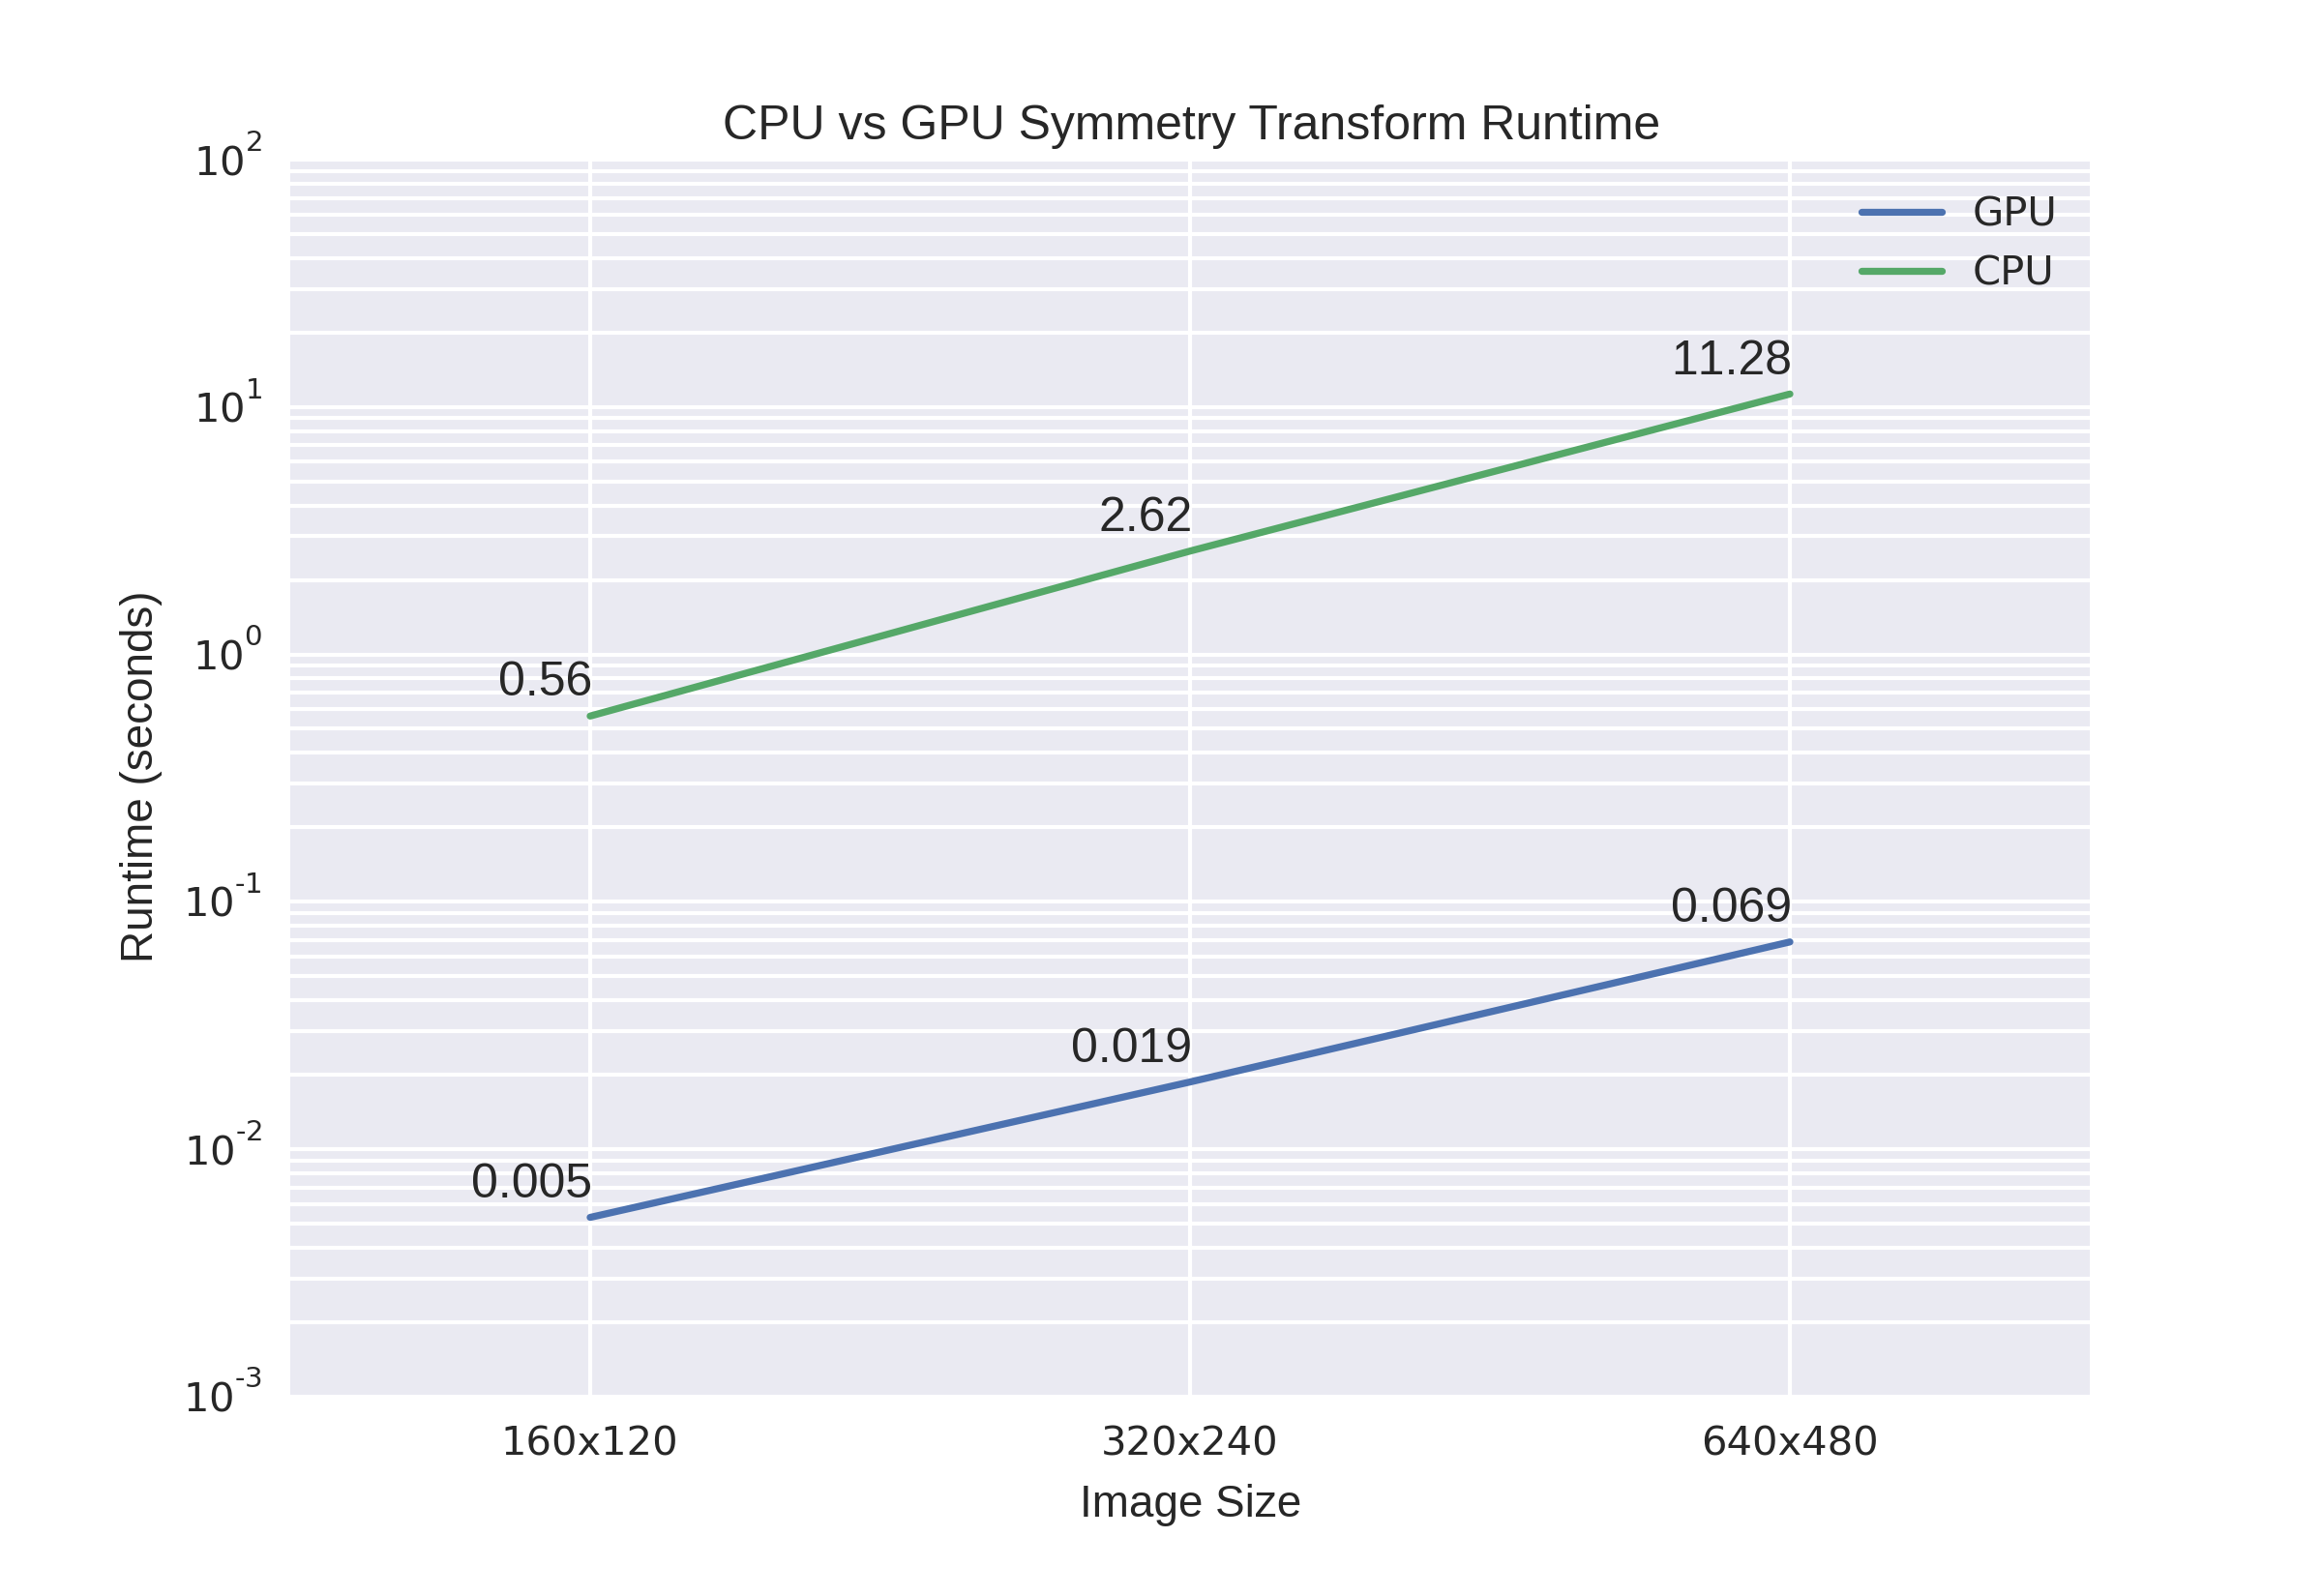
\includegraphics[width=0.6\linewidth]{figures/cpu_v_gpu.png}
\caption{\label{fig:perf}
Single-\gls{cpu} vs \gls{gpu} performance comparison. Note that there is two orders of magnitude improvement between the \gls{gpu} and the \gls{cpu} runtime. Tests were performed on an Intel 4th-Gen Core i7 2.9 GHz processor and NVidia Quadro M3000M \gls{gpu} with 768 CUDA cores}
\end{figure}

\subsection{Transform Output}
\label{sec:transform-output}

For our purposes, we are much less interested in the symmetry direction as we are in the symmetry magnitude (as discussed in the introduction). \Arlfig{fig:ex_xforms} shows example output from the implemented symmetry transform as well as simple "feature" detection output derived from the symmetry magnitude images. A quick and dirty method for finding features is to use non-maximum suppression to find local maxima (and then suppress any other maxima within a given radius). To show the usefulness of the transform on natural images, we implemented a simple detector that computes an image pyramid, runs the symmetry transform on each layer, and then merges the result into a single full-scale magnitude image in order to find local maxima. In the results shown, our detector uses a suppression radius of 15 pixels. 

\Needspace{0.8\textheight}
\begin{figure}[ht]
\centering
\begin{subfigure}[]{0.25\linewidth}\label{fig:kit_smag_0}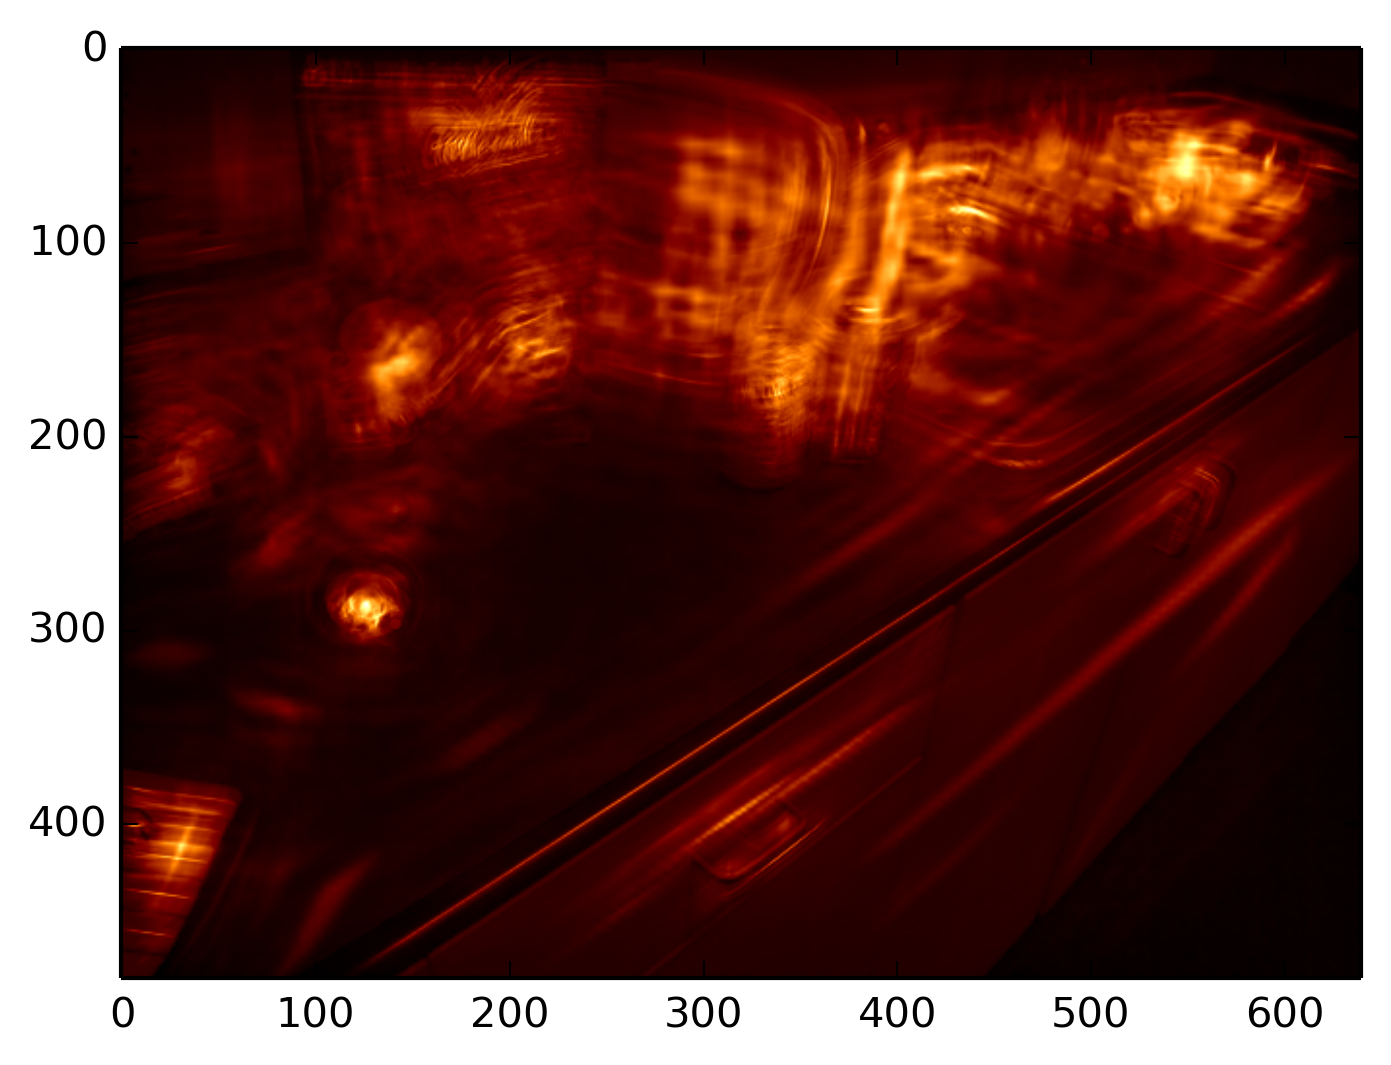
\includegraphics[width=\linewidth]{figures/kitchen_smag_1}\end{subfigure}%
\begin{subfigure}[]{0.25\linewidth}\label{fig:kit_feats_0}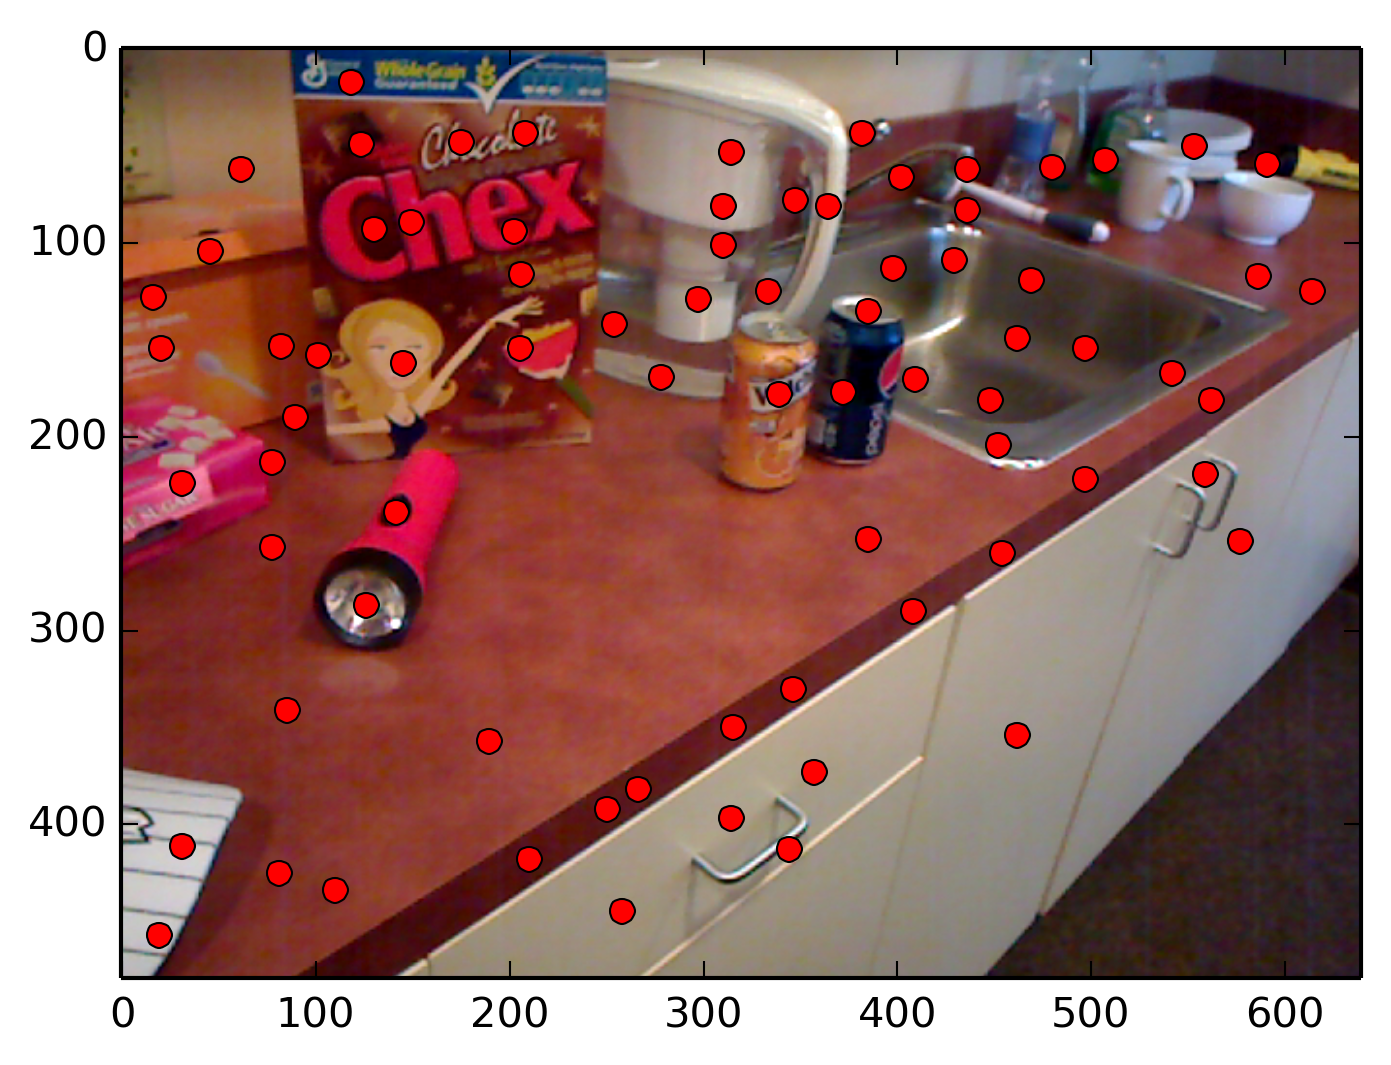
\includegraphics[width=\linewidth]{figures/kitchen_feats_1}\end{subfigure}%
\begin{subfigure}[]{0.25\linewidth}\label{fig:meet_smag_0}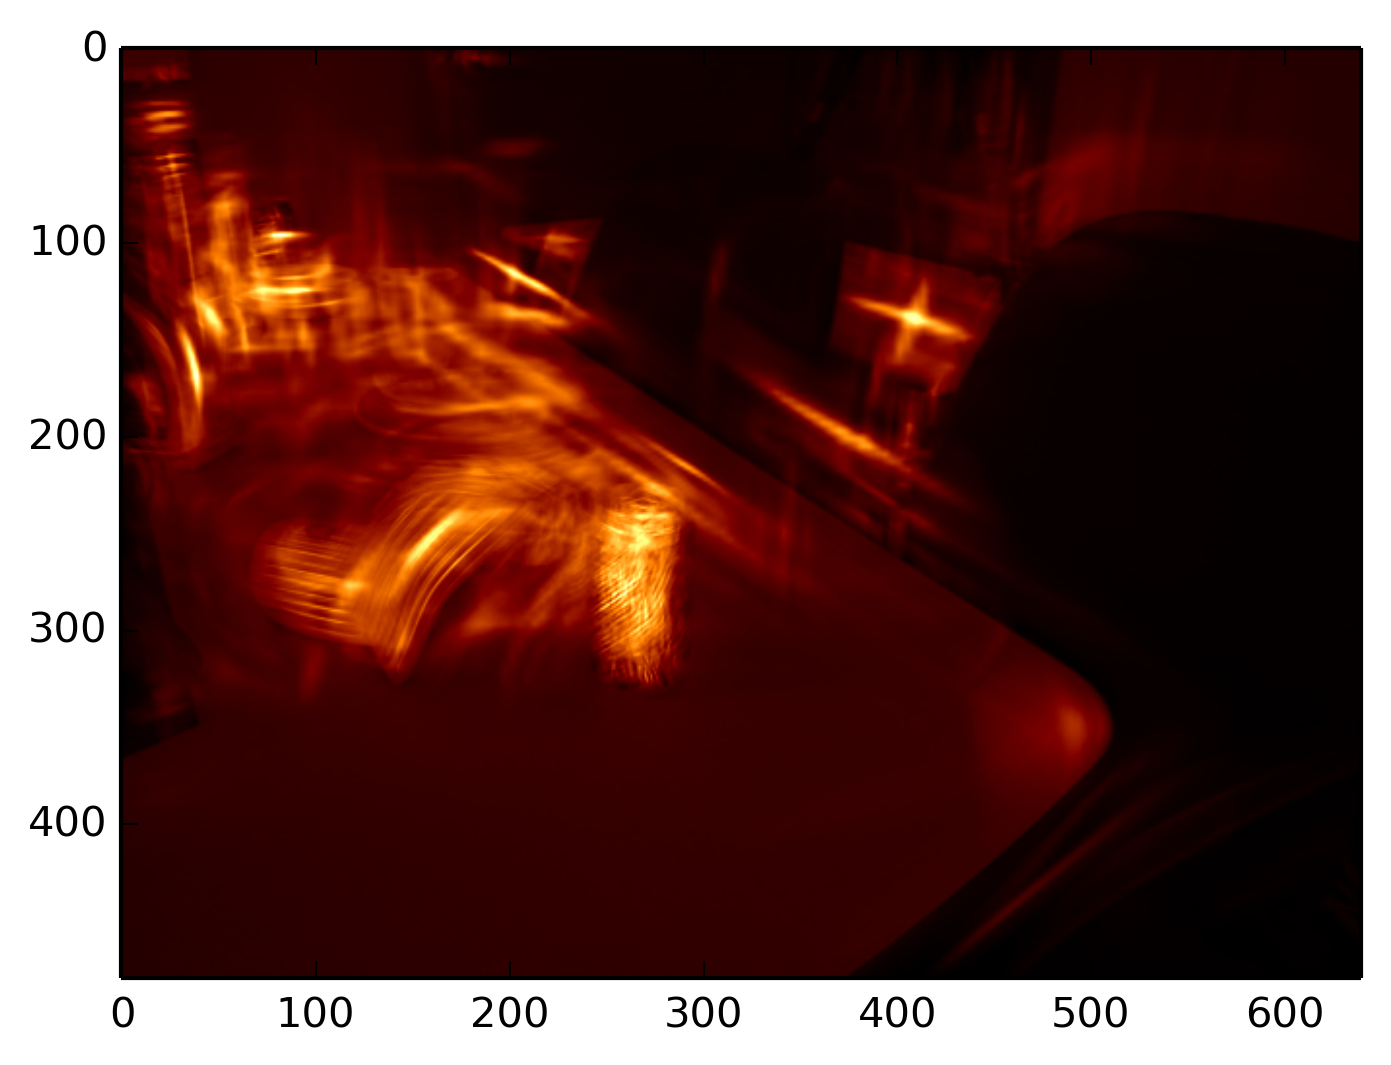
\includegraphics[width=\linewidth]{figures/meeting_smag_1}\end{subfigure}%
\begin{subfigure}[]{0.25\linewidth}\label{fig:meet_feats_0}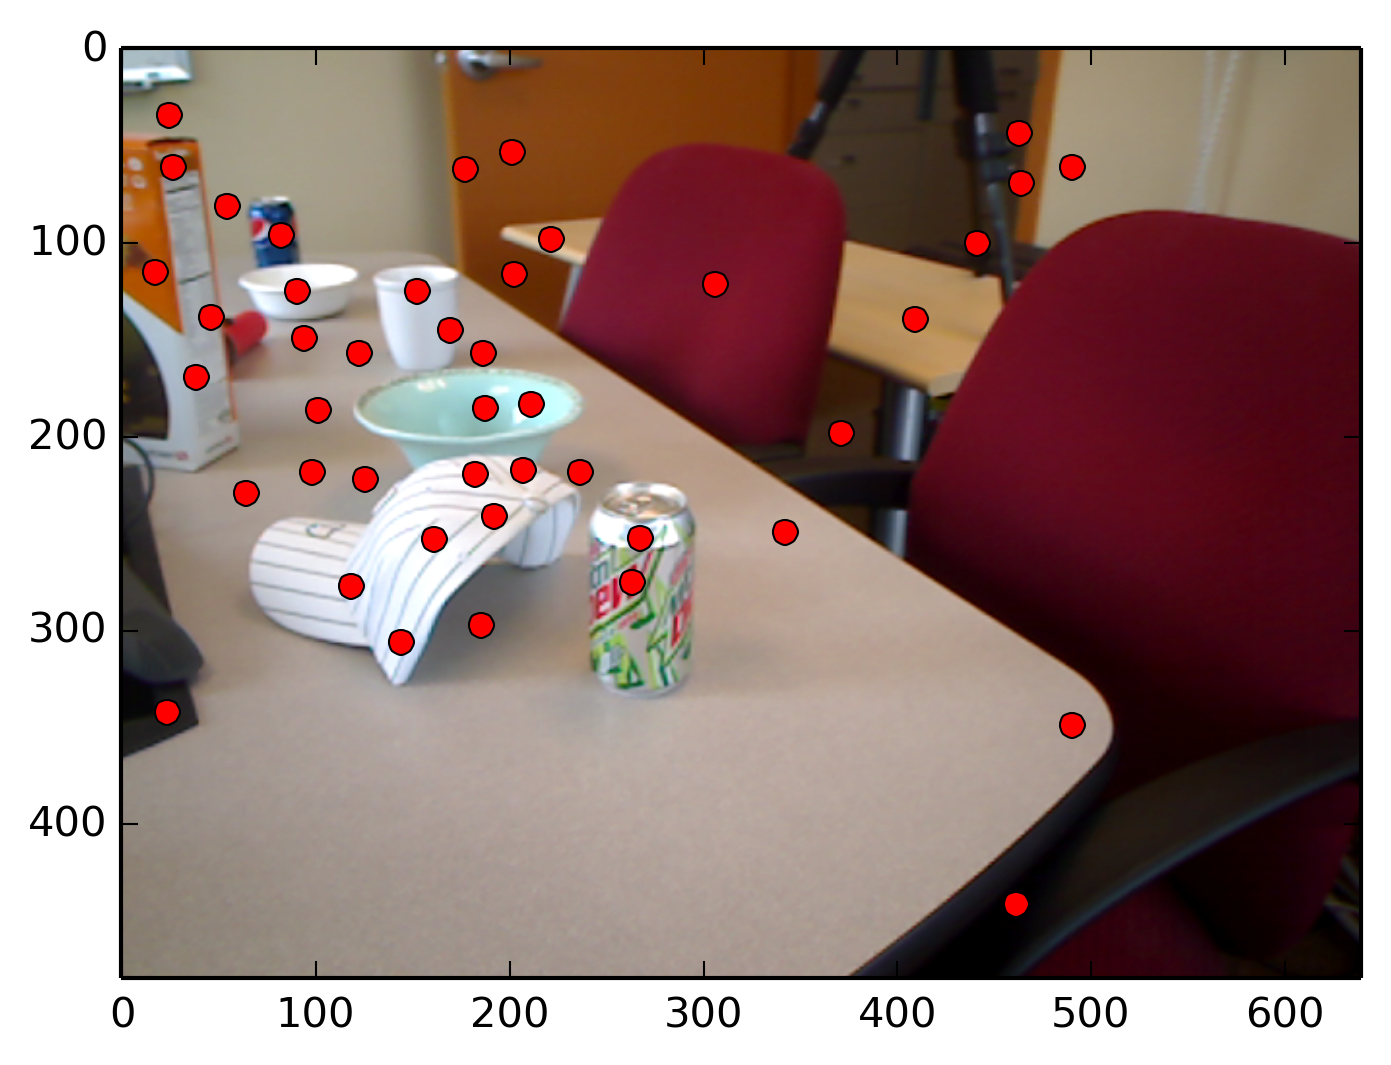
\includegraphics[width=\linewidth]{figures/meeting_feats_1}\end{subfigure}\\
\begin{subfigure}[]{0.25\linewidth}\label{fig:kit_smag_1}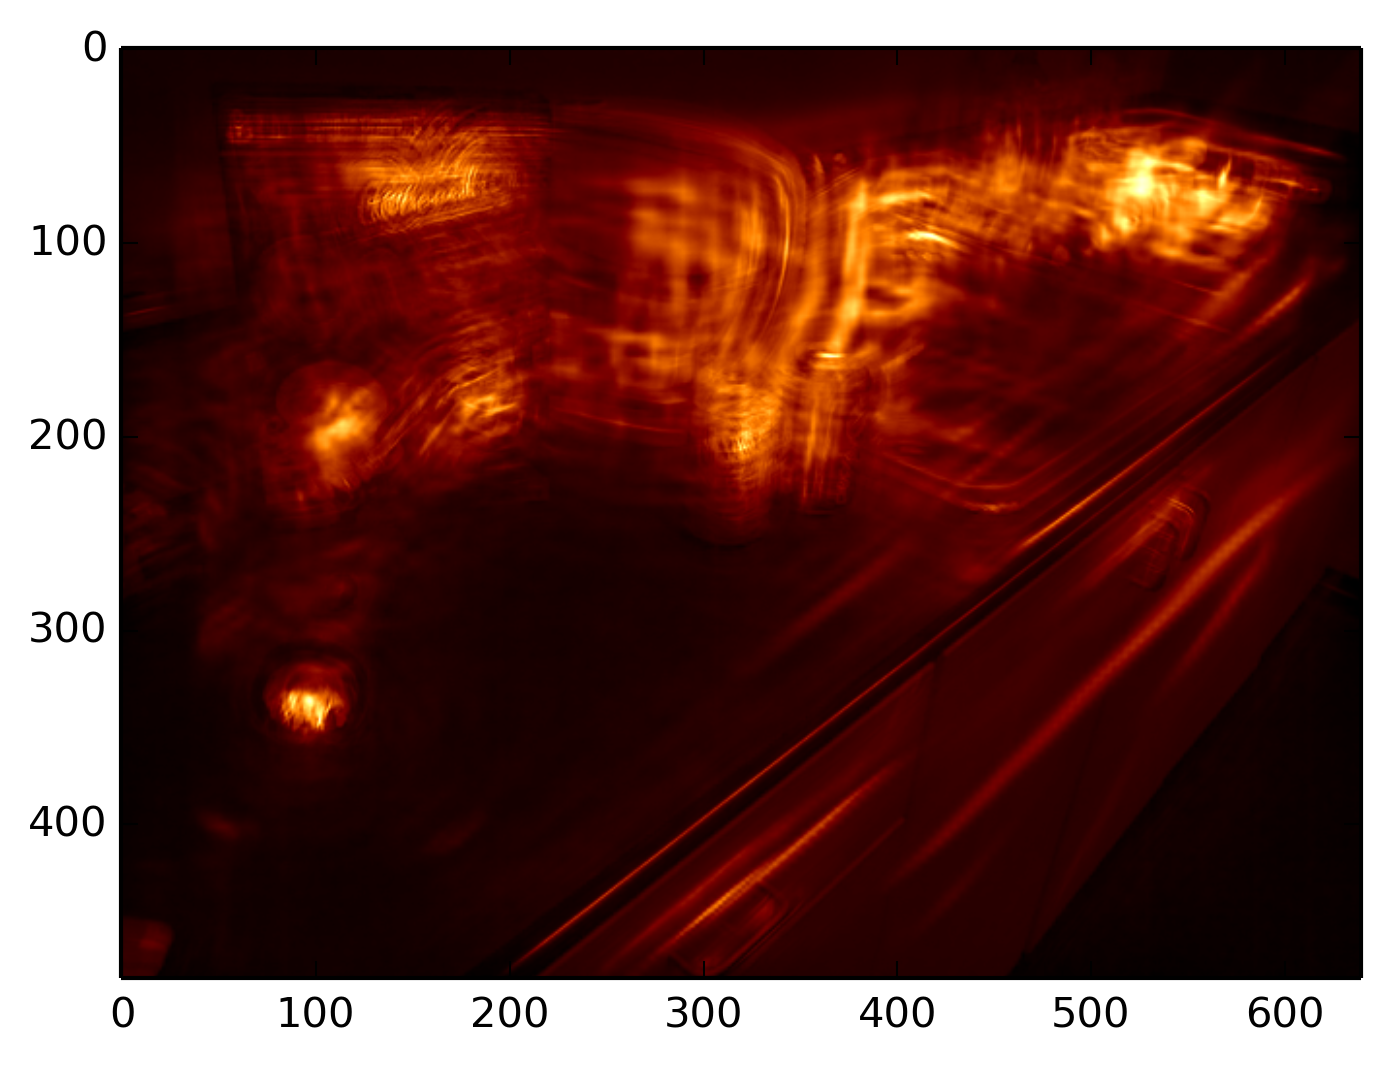
\includegraphics[width=\linewidth]{figures/kitchen_smag_3}\end{subfigure}%
\begin{subfigure}[]{0.25\linewidth}\label{fig:kit_feats_1}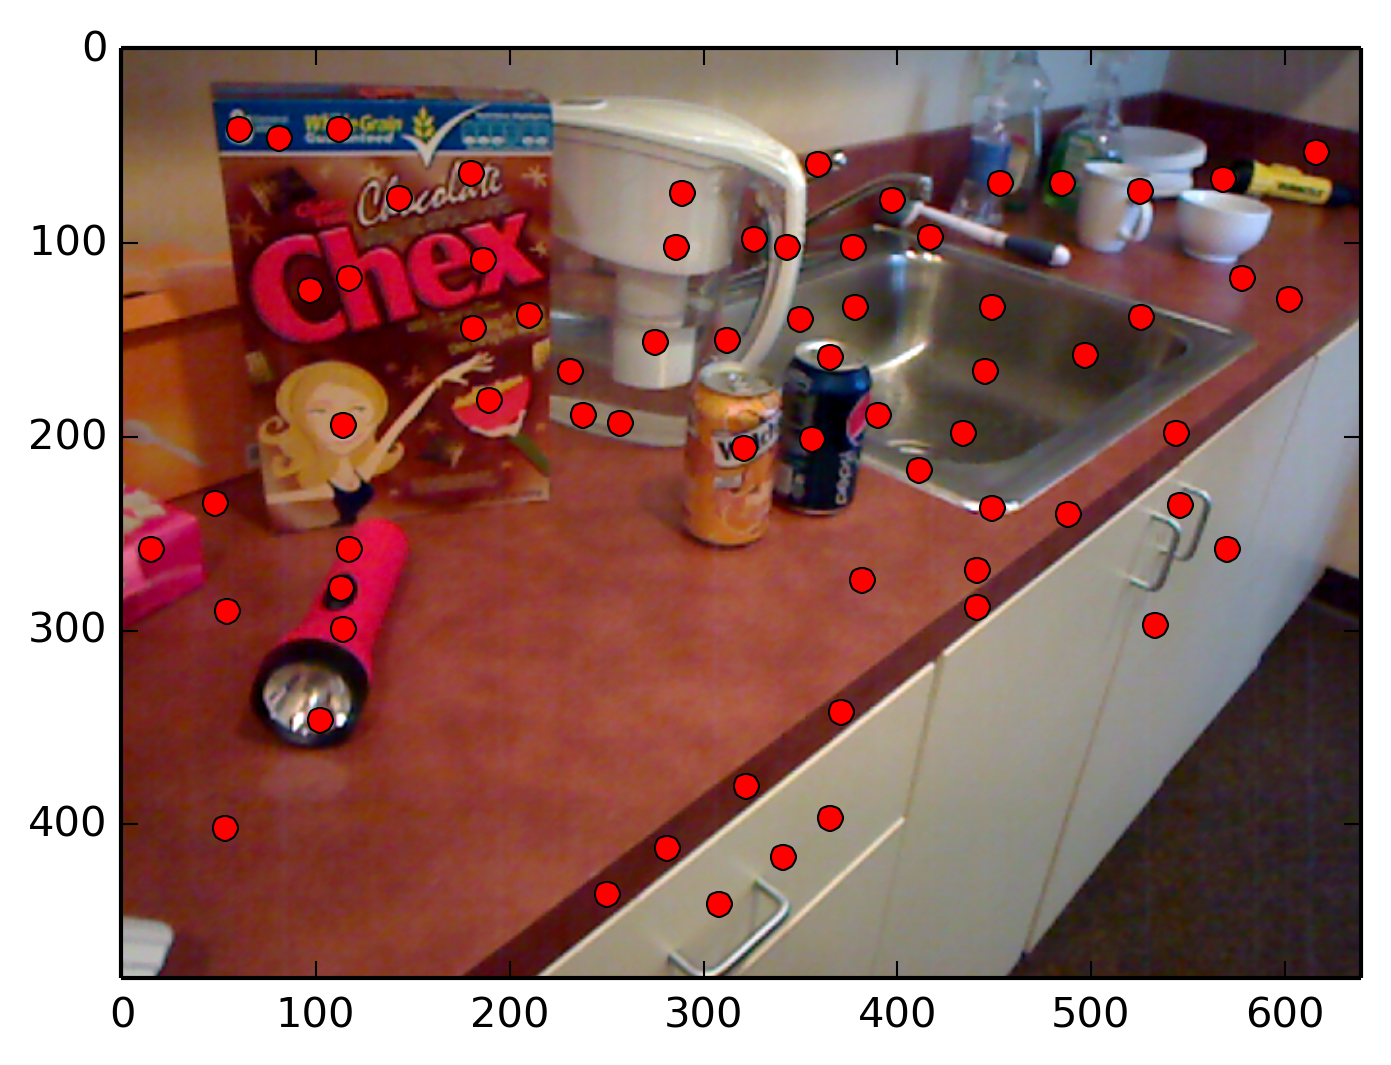
\includegraphics[width=\linewidth]{figures/kitchen_feats_3}\end{subfigure}%
\begin{subfigure}[]{0.25\linewidth}\label{fig:meet_smag_1}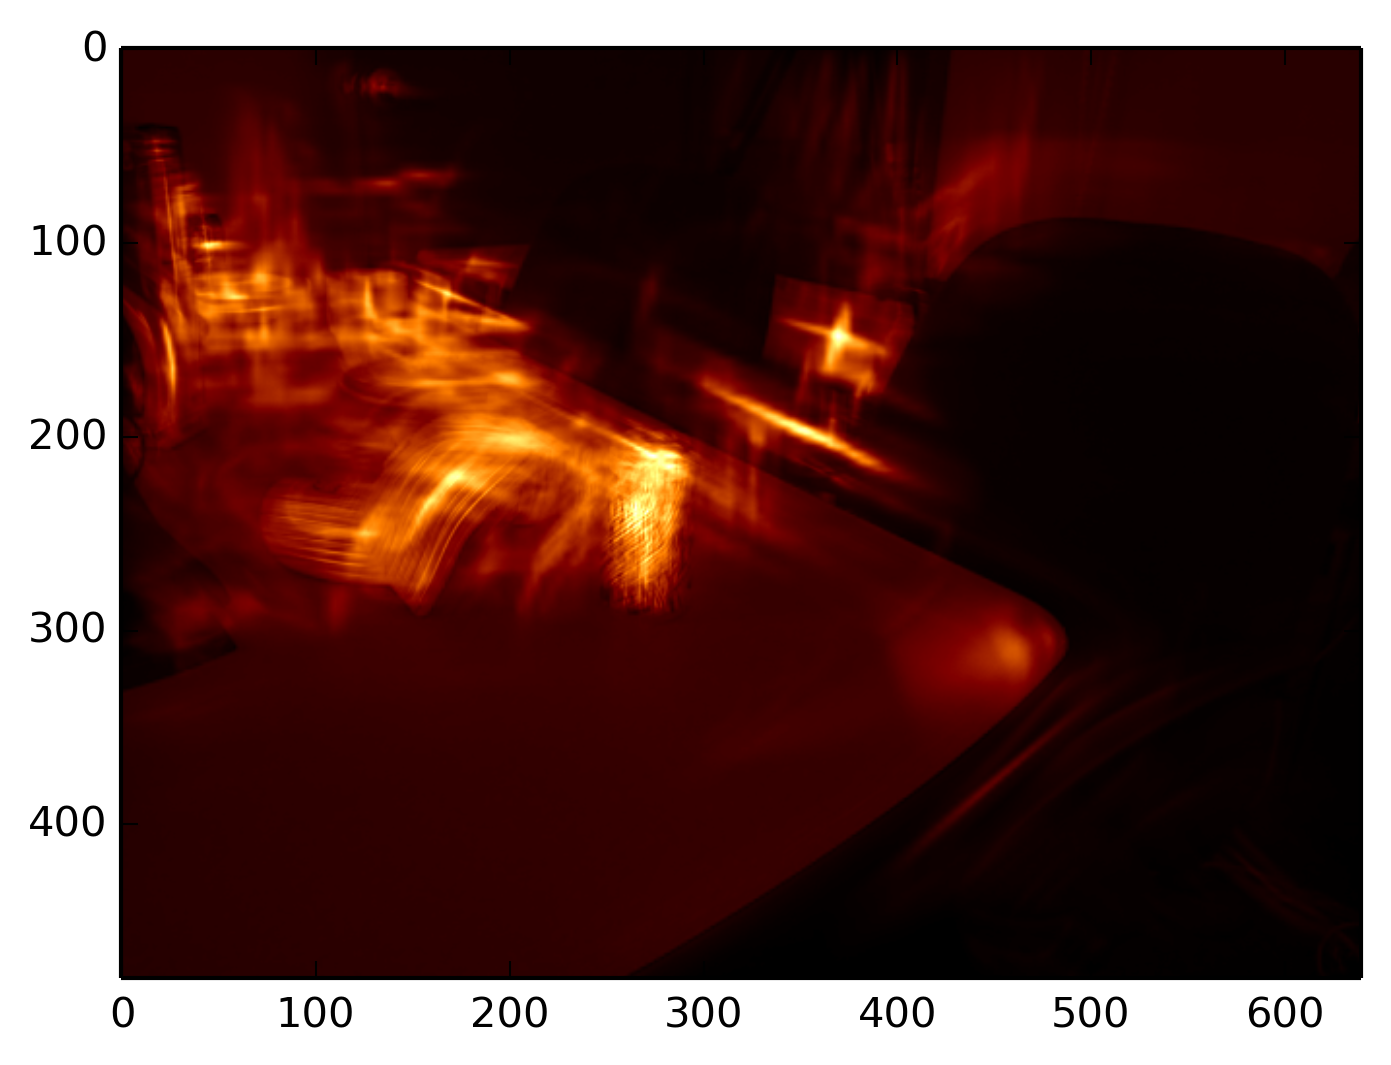
\includegraphics[width=\linewidth]{figures/meeting_smag_3}\end{subfigure}%
\begin{subfigure}[]{0.25\linewidth}\label{fig:meet_feats_1}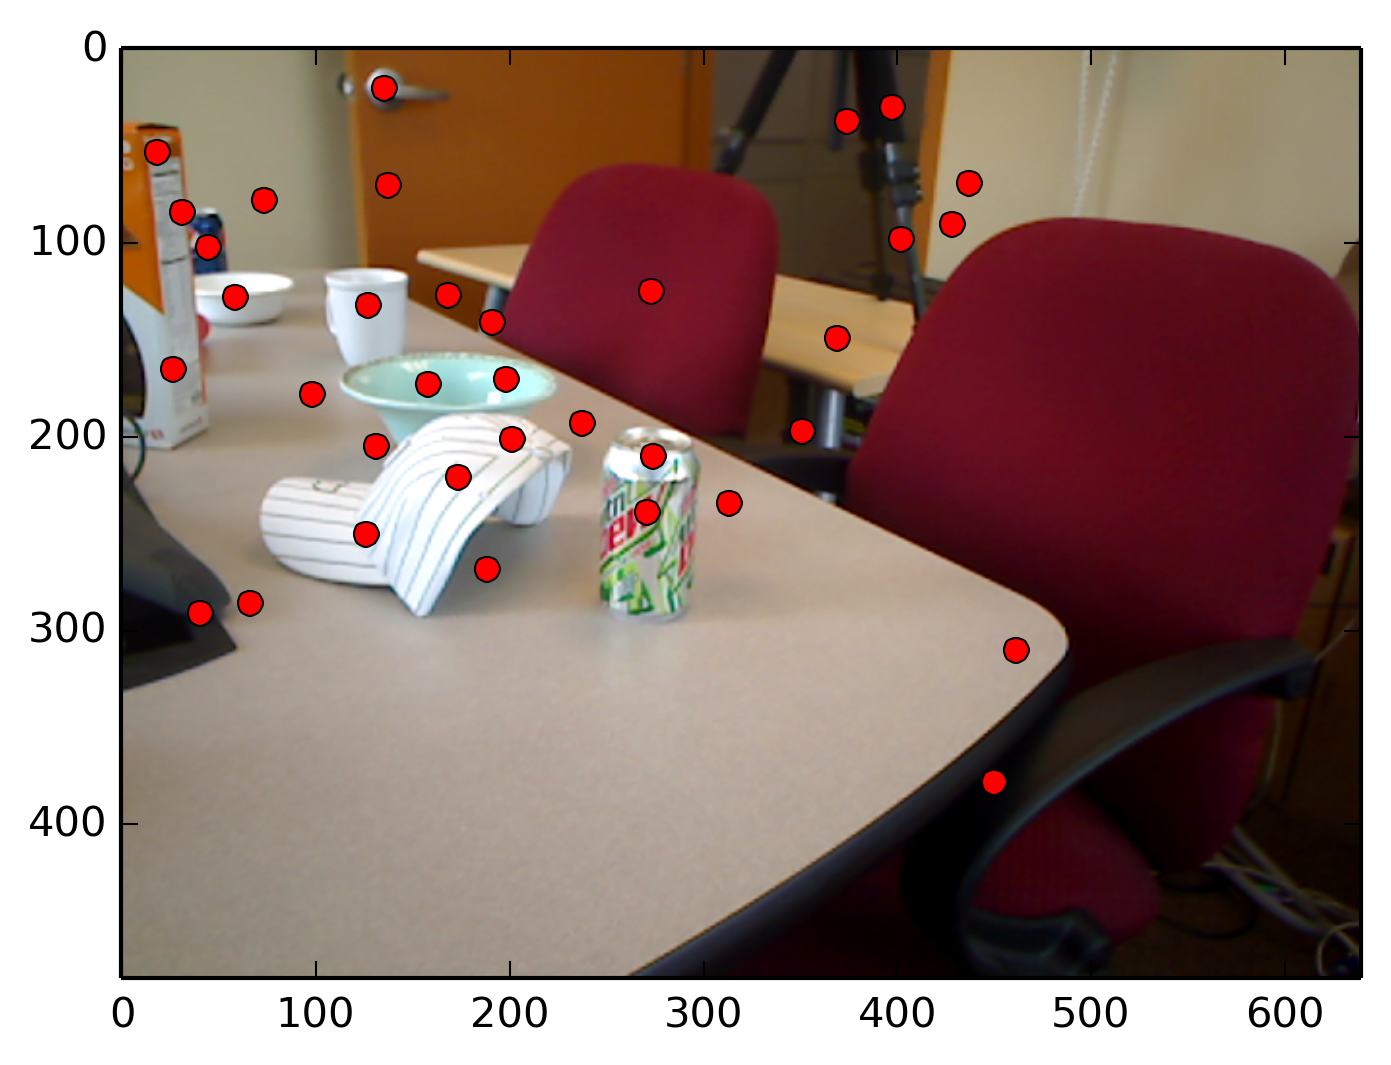
\includegraphics[width=\linewidth]{figures/meeting_feats_3}\end{subfigure}\\
\begin{subfigure}[]{0.25\linewidth}\label{fig:kit_smag_2}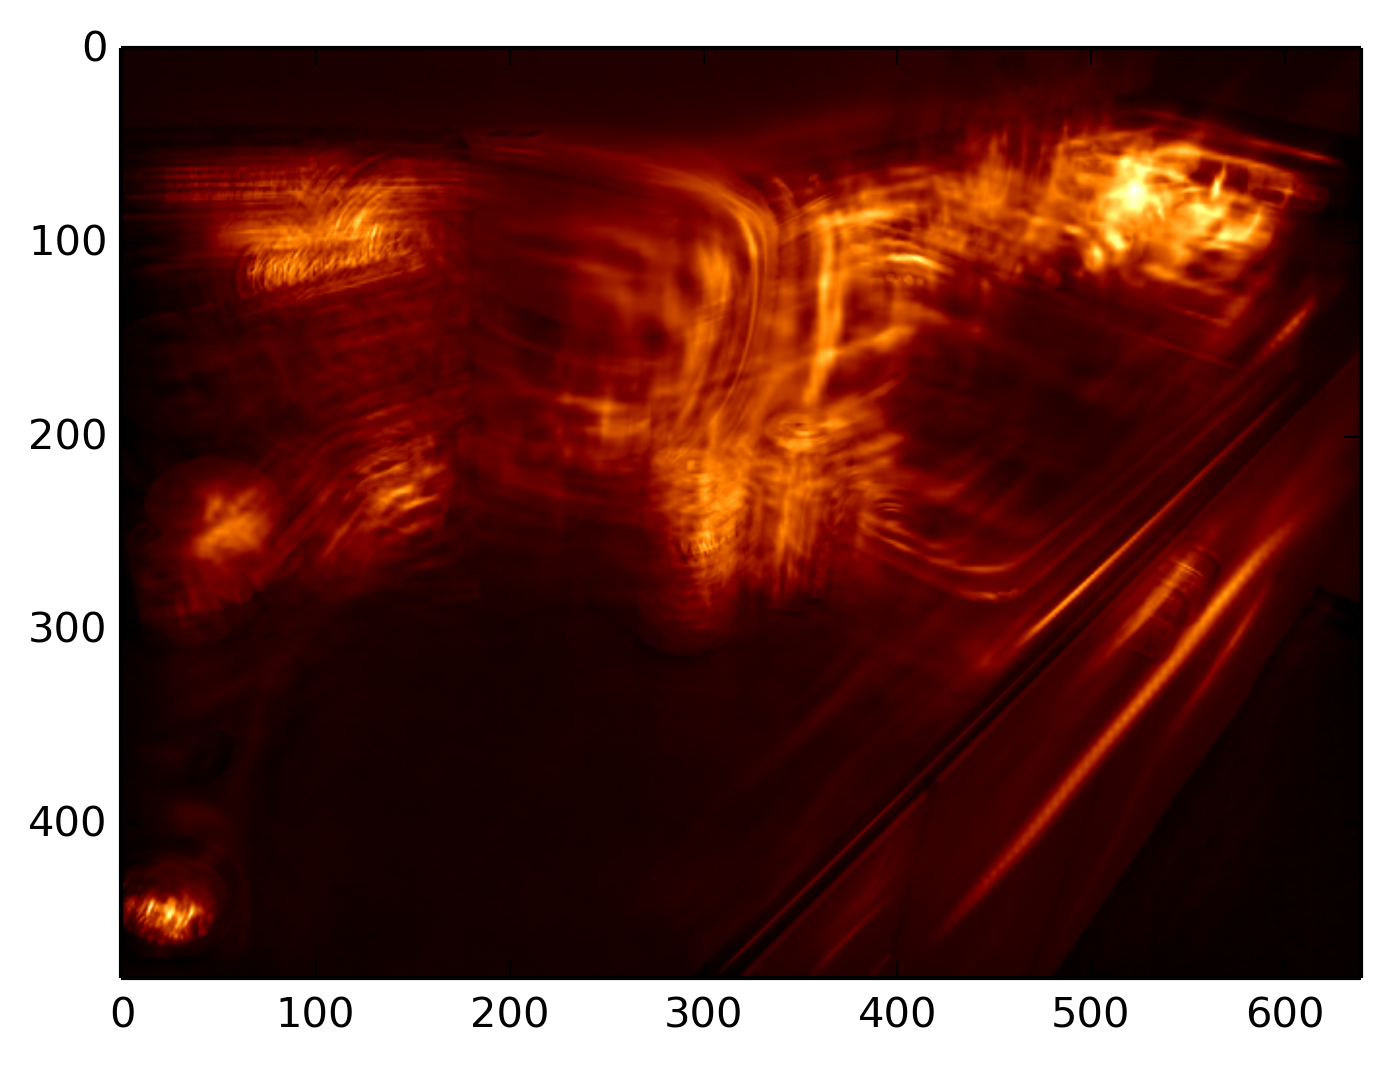
\includegraphics[width=\linewidth]{figures/kitchen_smag_5}\end{subfigure}%
\begin{subfigure}[]{0.25\linewidth}\label{fig:kit_feats_2}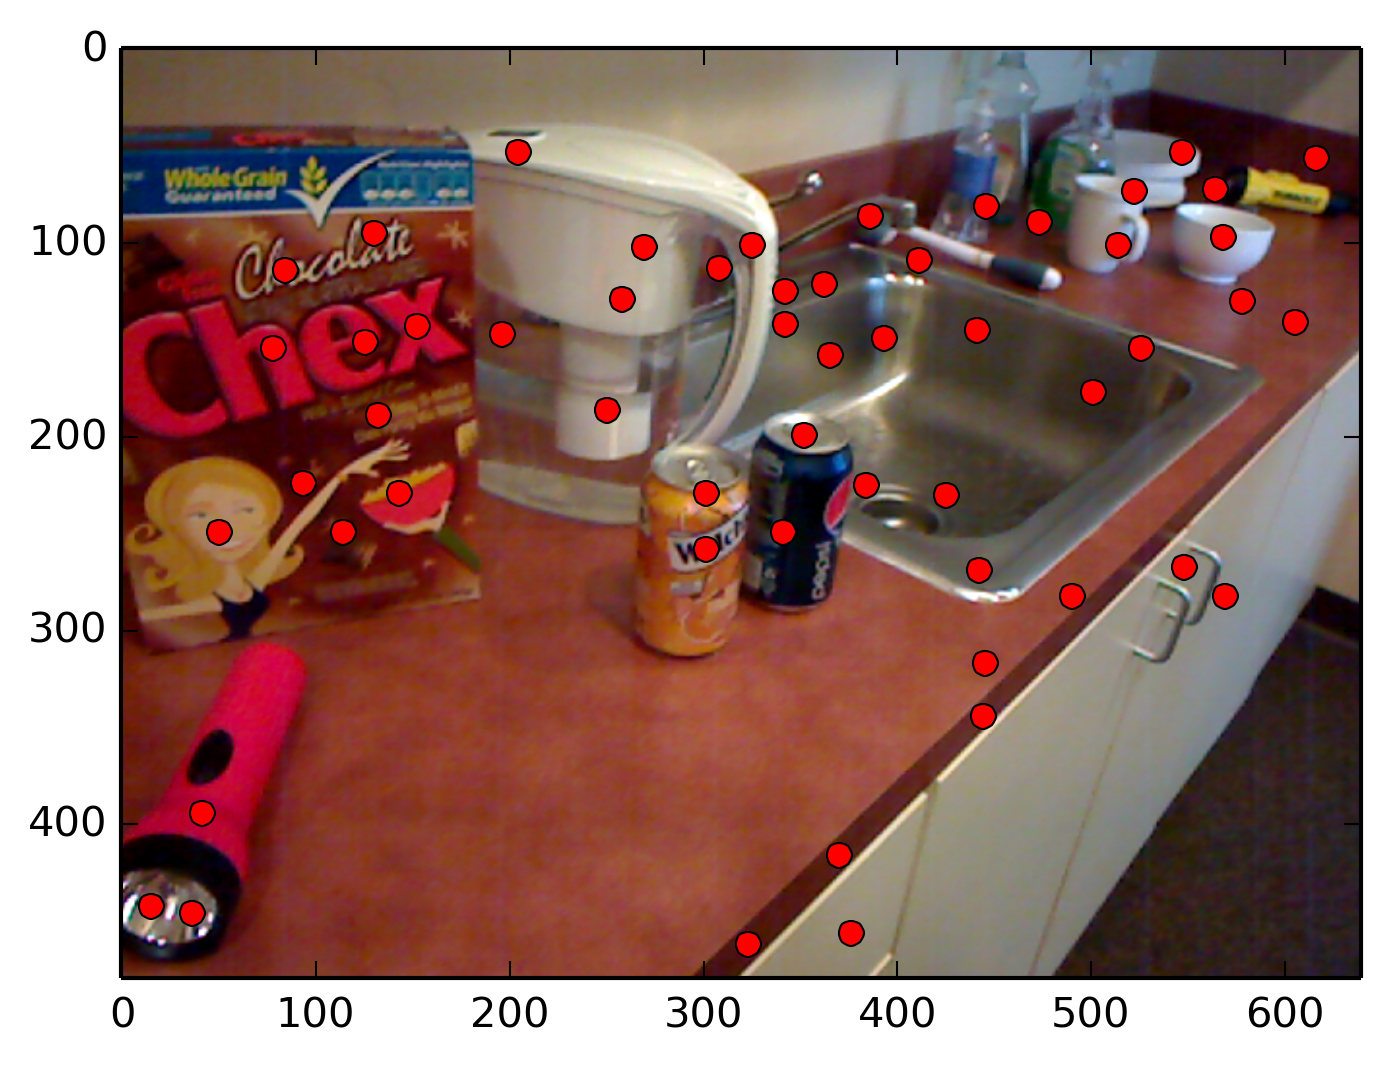
\includegraphics[width=\linewidth]{figures/kitchen_feats_5}\end{subfigure}%
\begin{subfigure}[]{0.25\linewidth}\label{fig:meet_smag_2}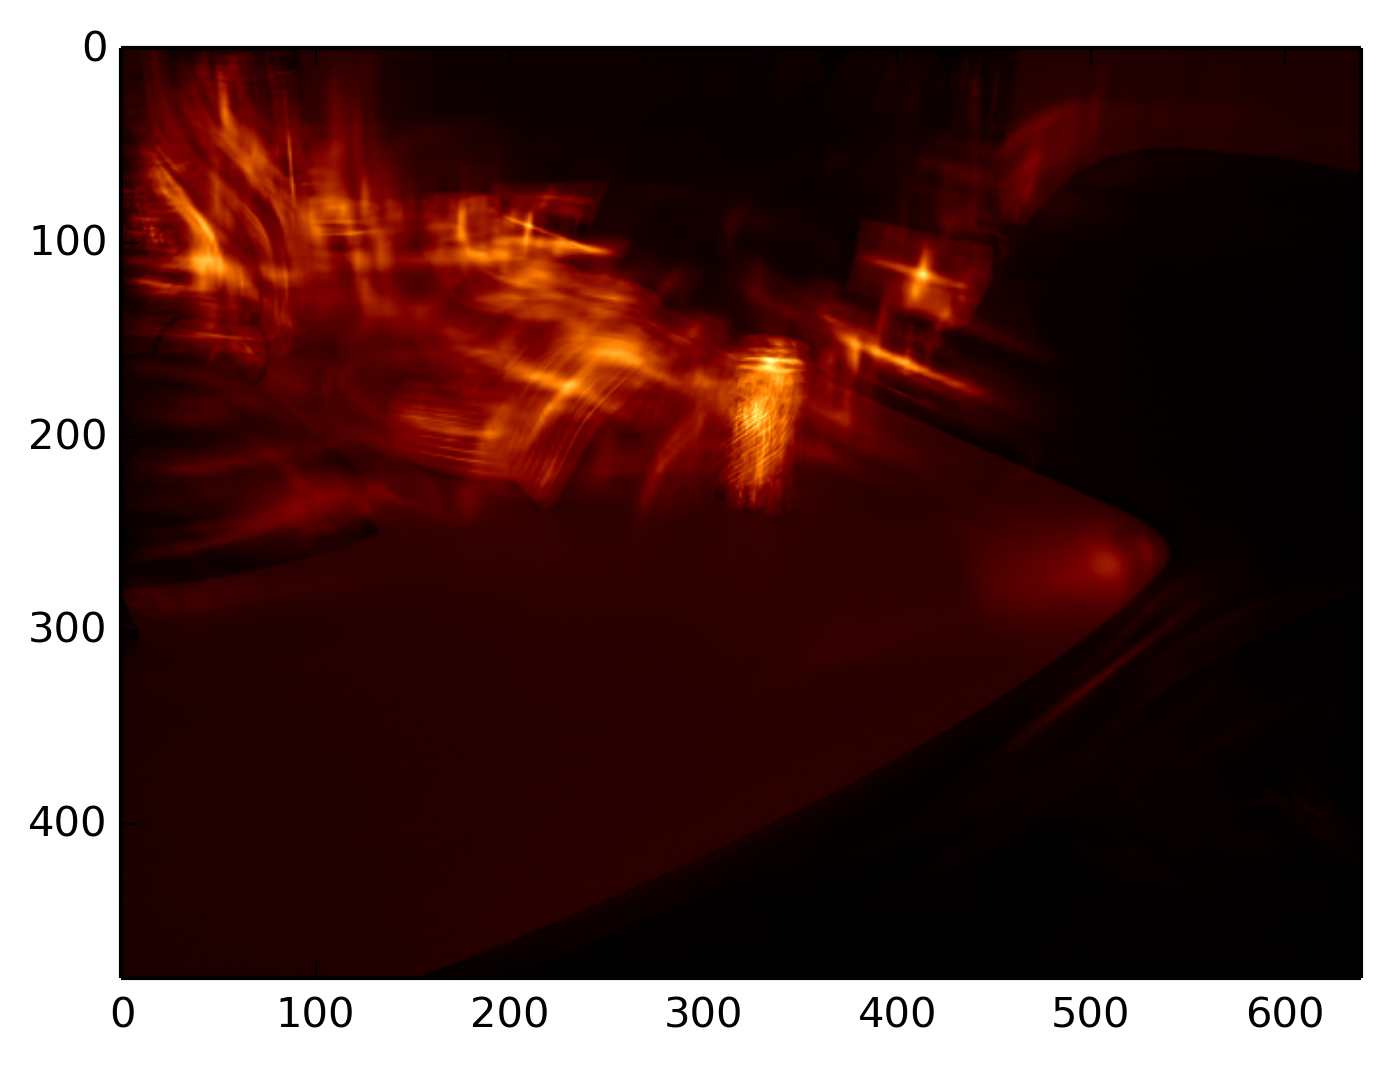
\includegraphics[width=\linewidth]{figures/meeting_smag_5}\end{subfigure}%
\begin{subfigure}[]{0.25\linewidth}\label{fig:meet_feats_2}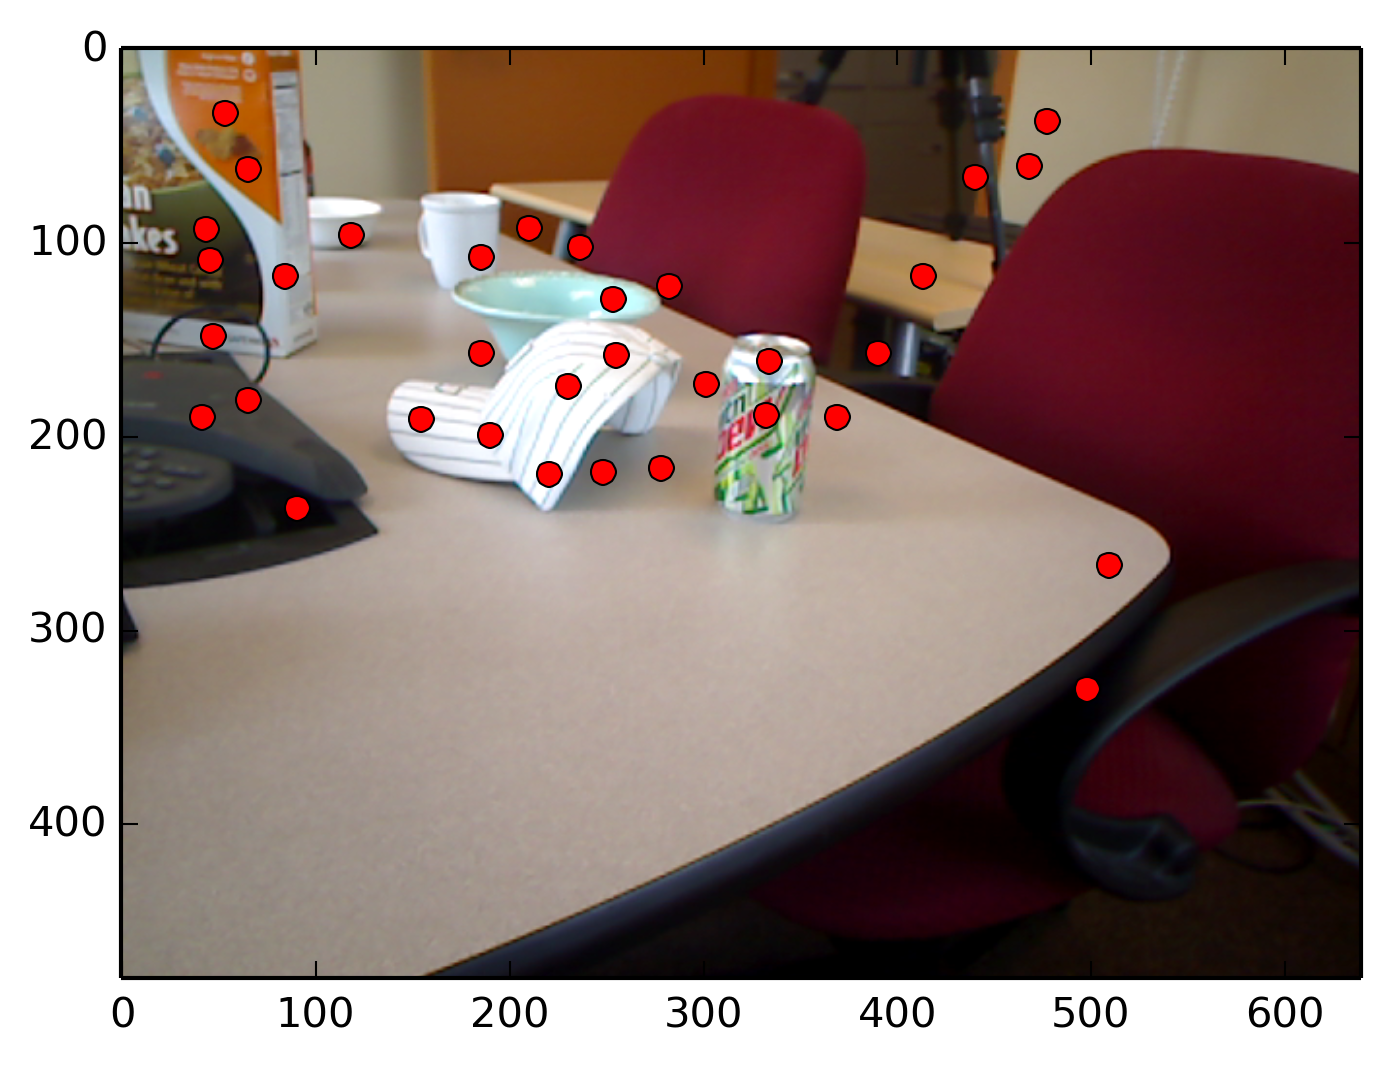
\includegraphics[width=\linewidth]{figures/meeting_feats_5}\end{subfigure}\\
\begin{subfigure}[]{0.25\linewidth}\label{fig:kit_smag_3}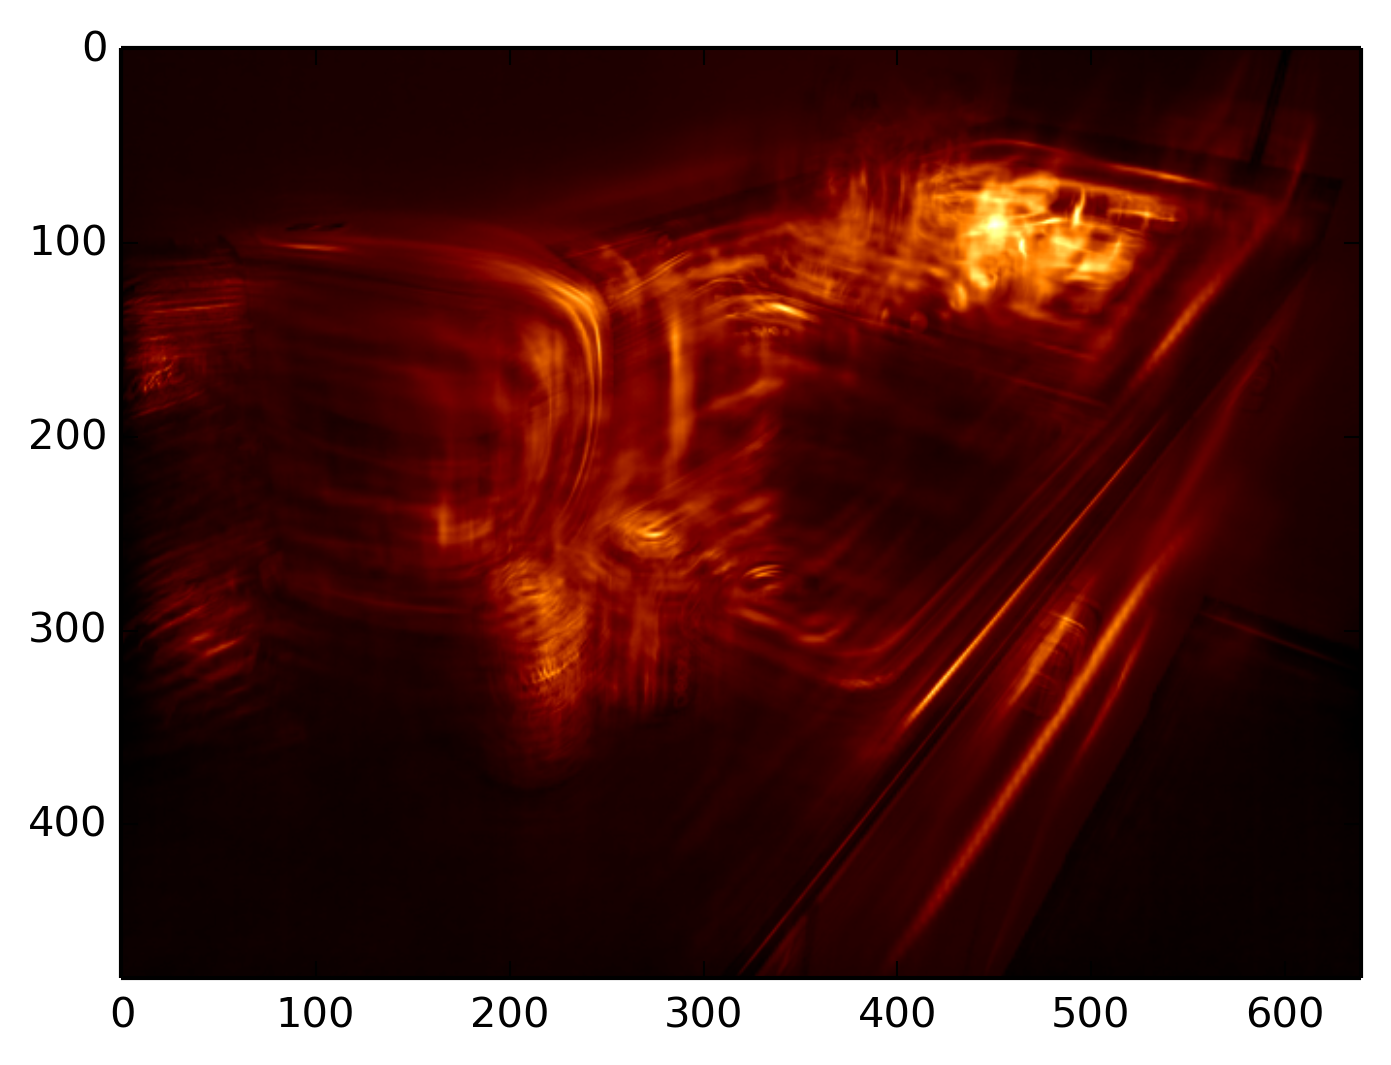
\includegraphics[width=\linewidth]{figures/kitchen_smag_7}\end{subfigure}%
\begin{subfigure}[]{0.25\linewidth}\label{fig:kit_feats_3}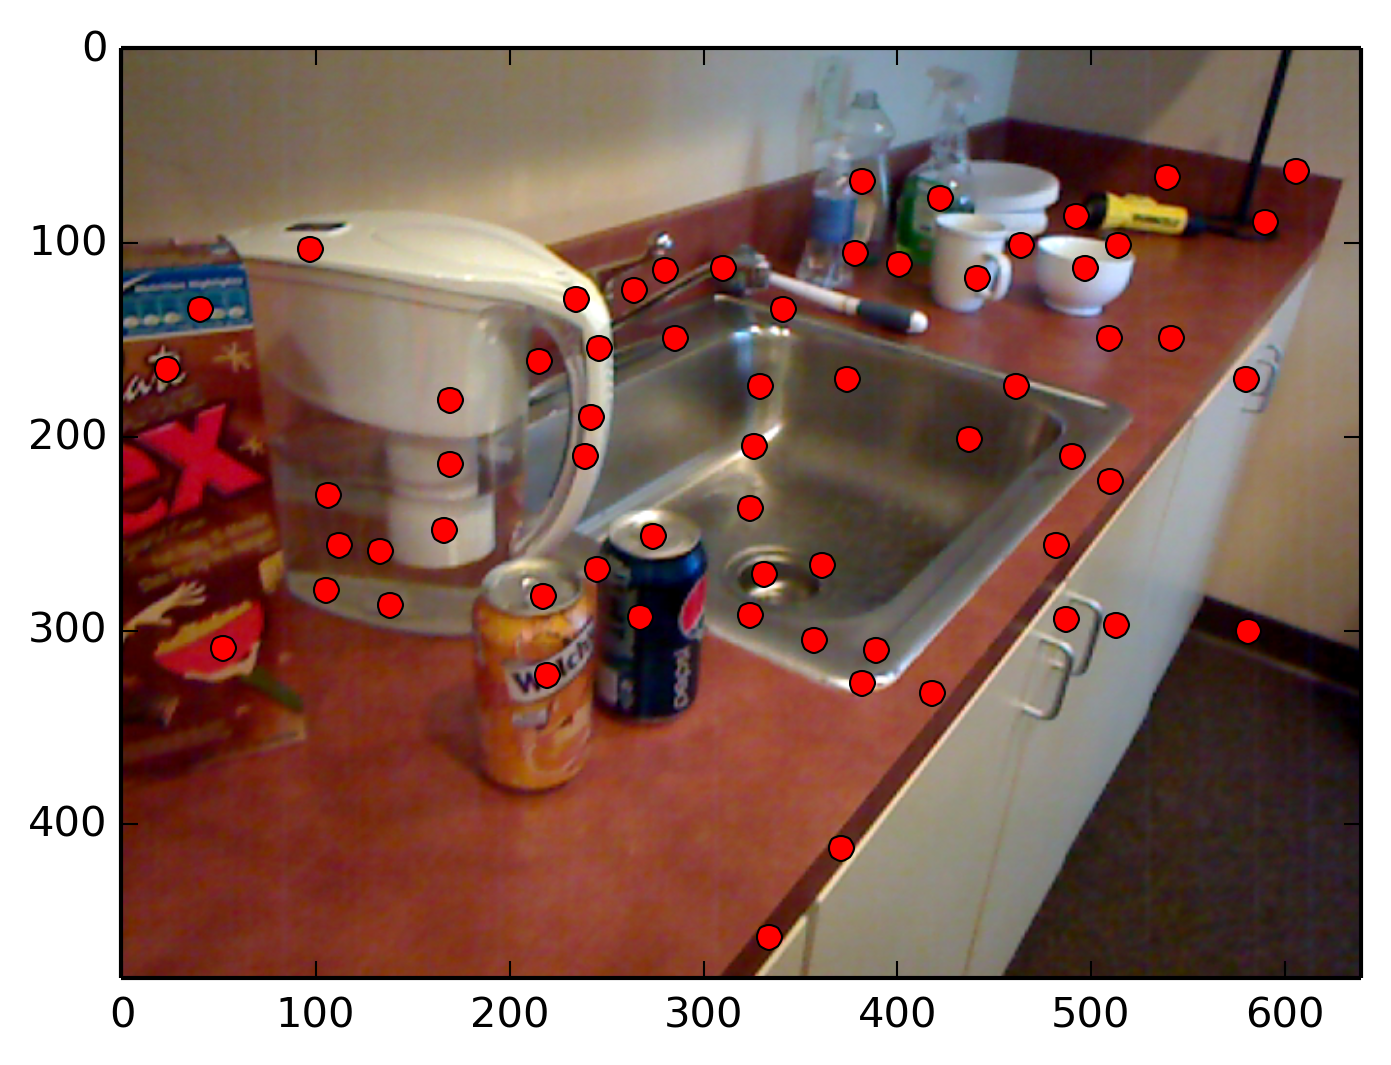
\includegraphics[width=\linewidth]{figures/kitchen_feats_7}\end{subfigure}%
\begin{subfigure}[]{0.25\linewidth}\label{fig:meet_smag_3}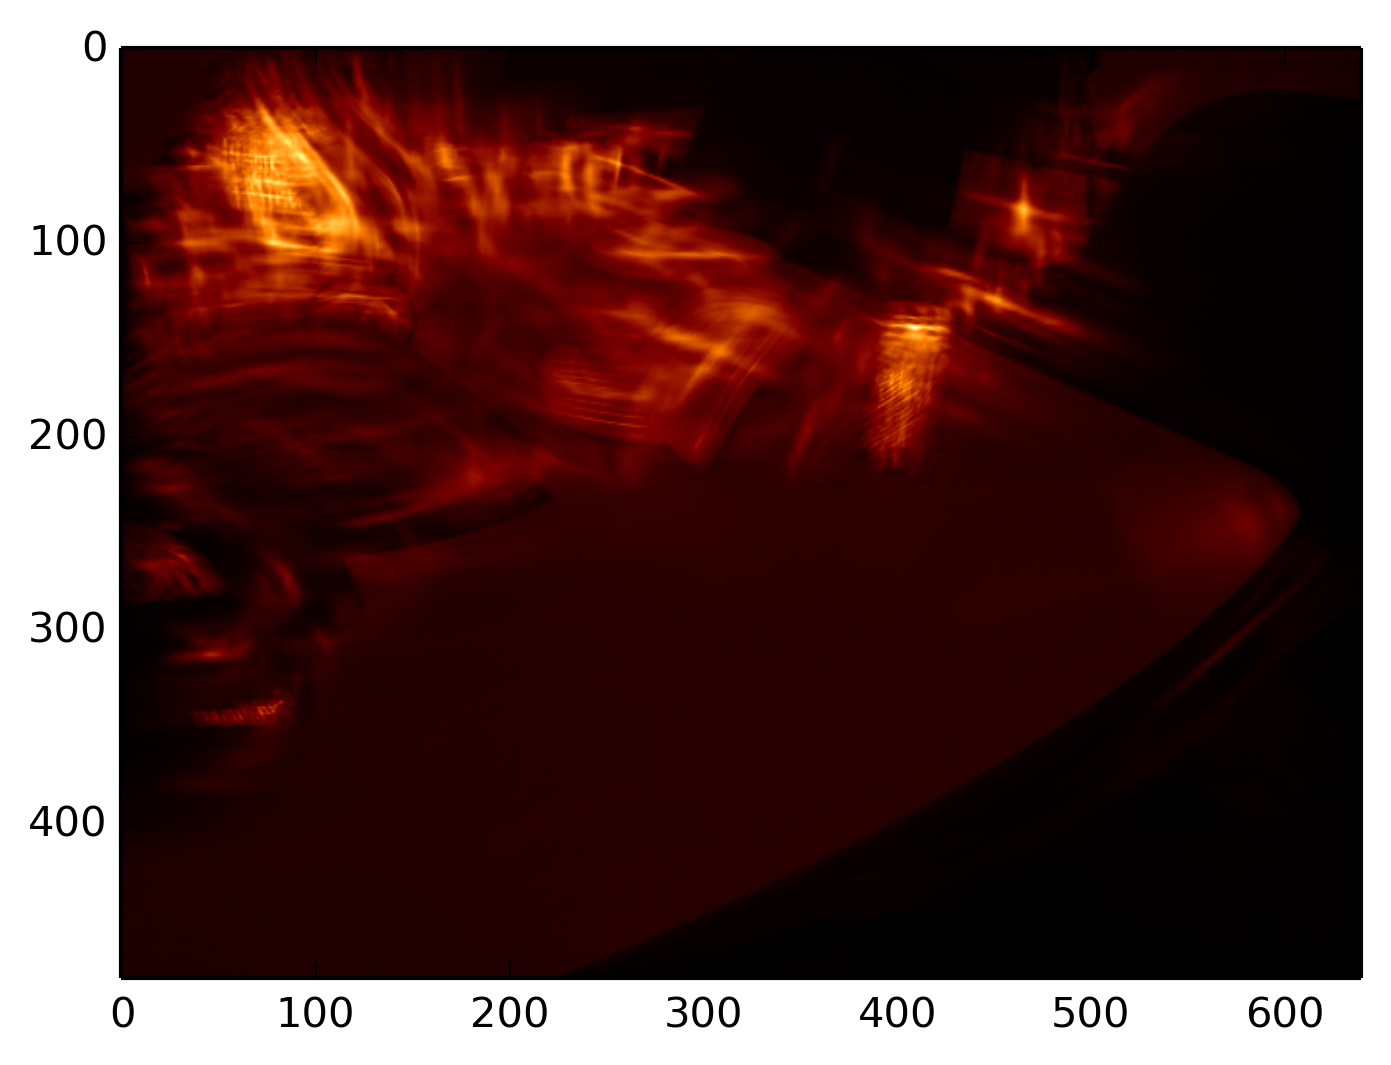
\includegraphics[width=\linewidth]{figures/meeting_smag_7}\end{subfigure}%
\begin{subfigure}[]{0.25\linewidth}\label{fig:meet_feats_3}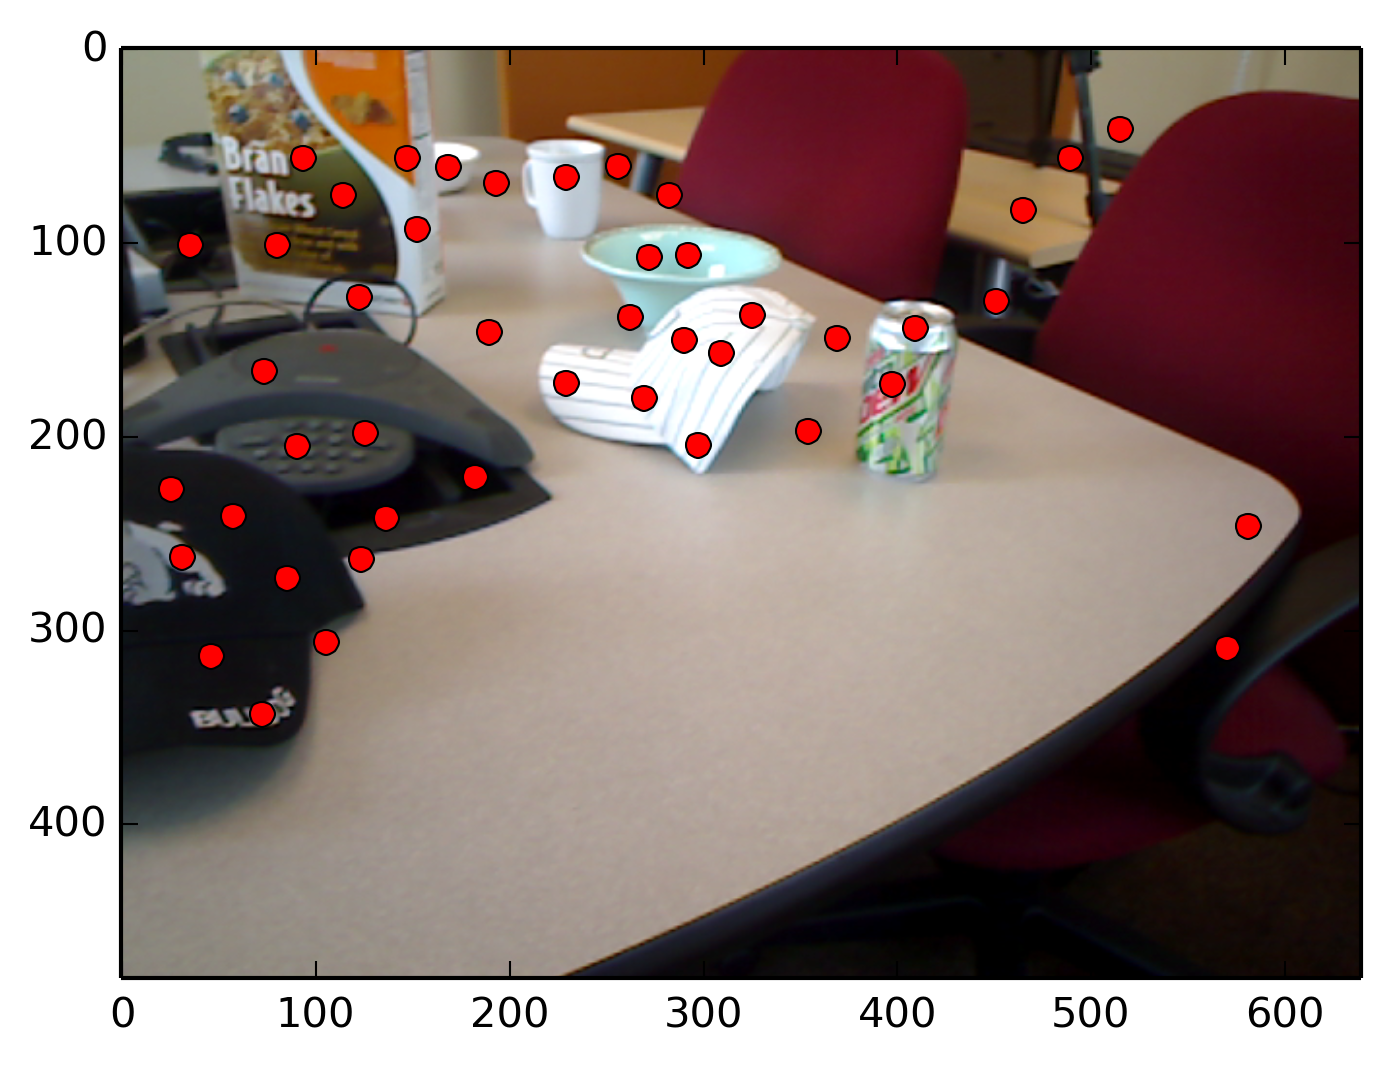
\includegraphics[width=\linewidth]{figures/meeting_feats_7}\end{subfigure}\\
\begin{subfigure}[]{0.25\linewidth}\label{fig:kit_smag_4}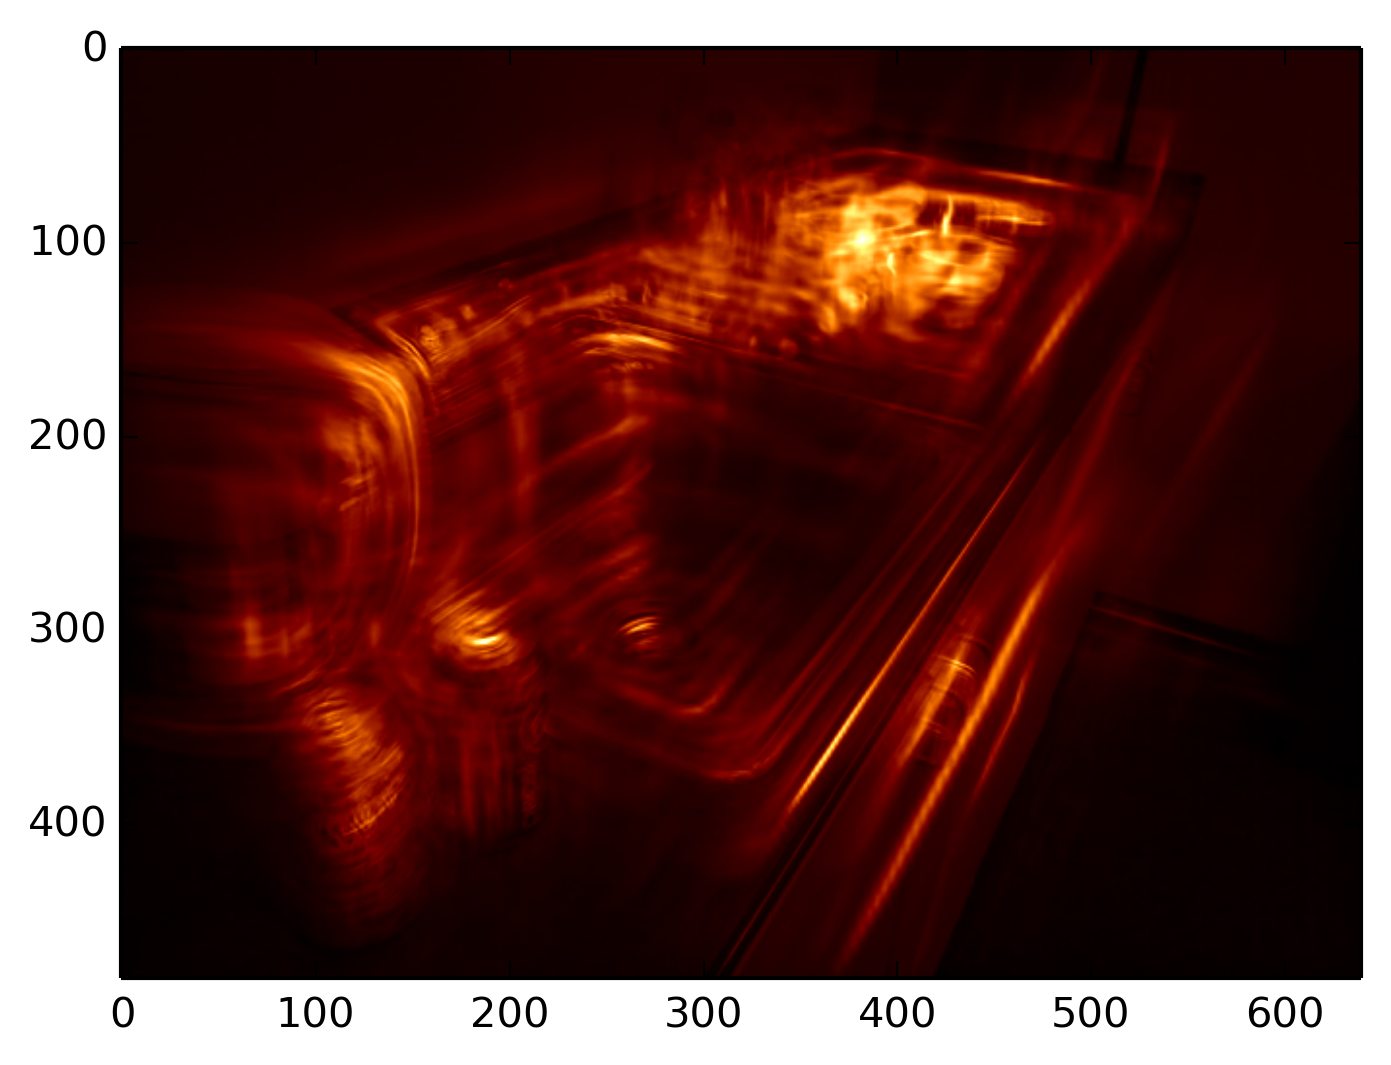
\includegraphics[width=\linewidth]{figures/kitchen_smag_9}\end{subfigure}%
\begin{subfigure}[]{0.25\linewidth}\label{fig:kit_feats_4}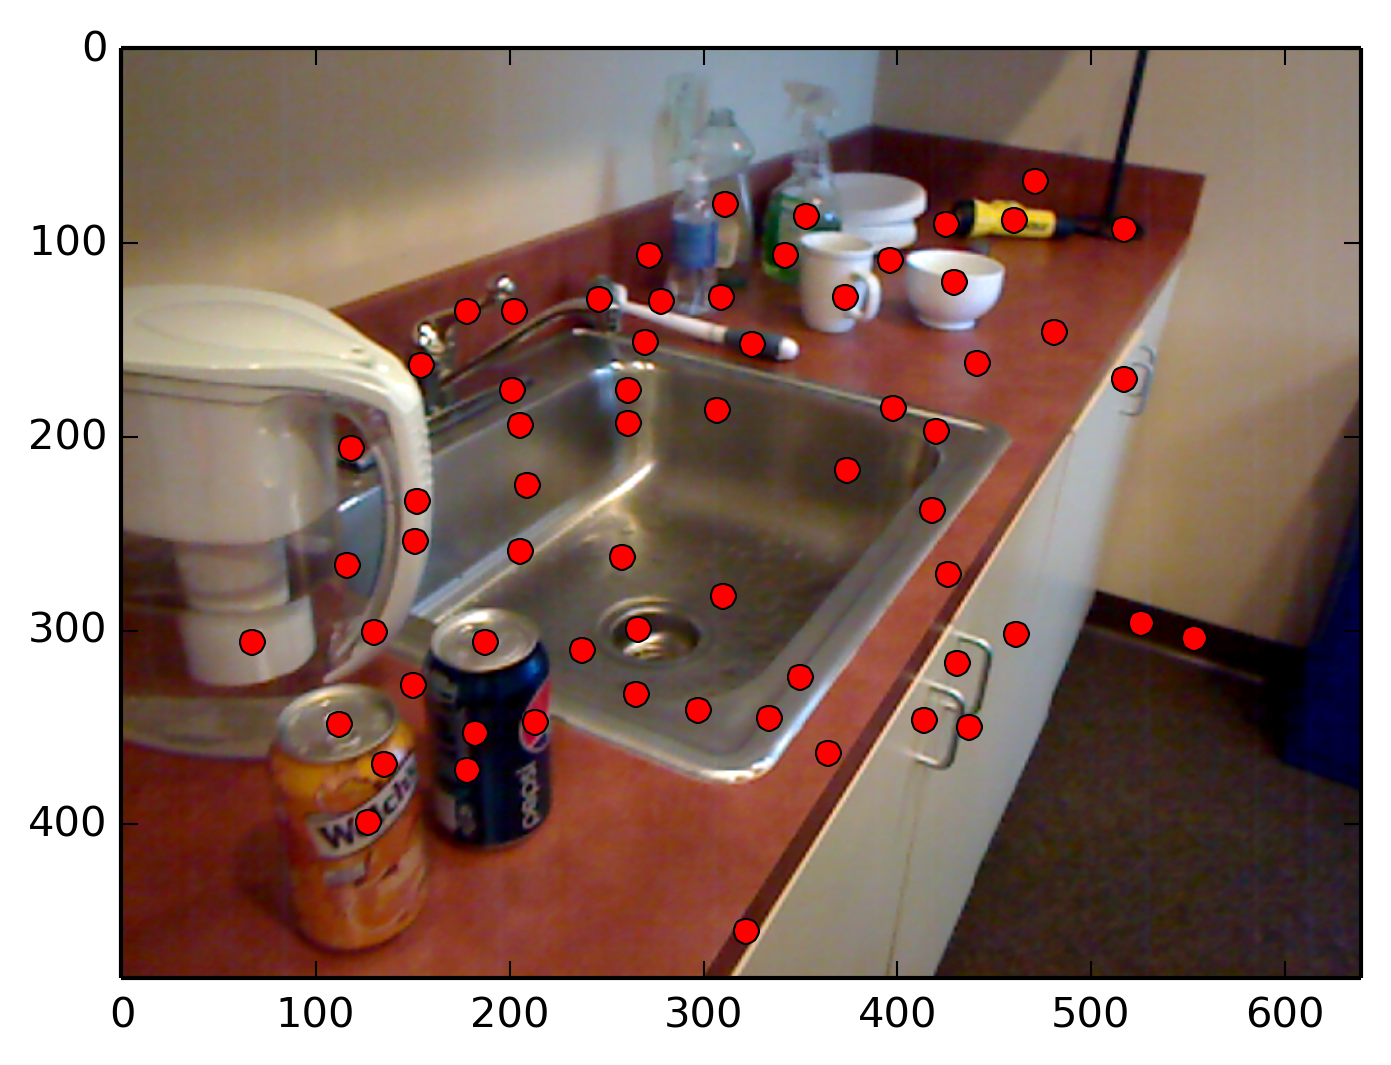
\includegraphics[width=\linewidth]{figures/kitchen_feats_9}\end{subfigure}%
\begin{subfigure}[]{0.25\linewidth}\label{fig:meet_smag_4}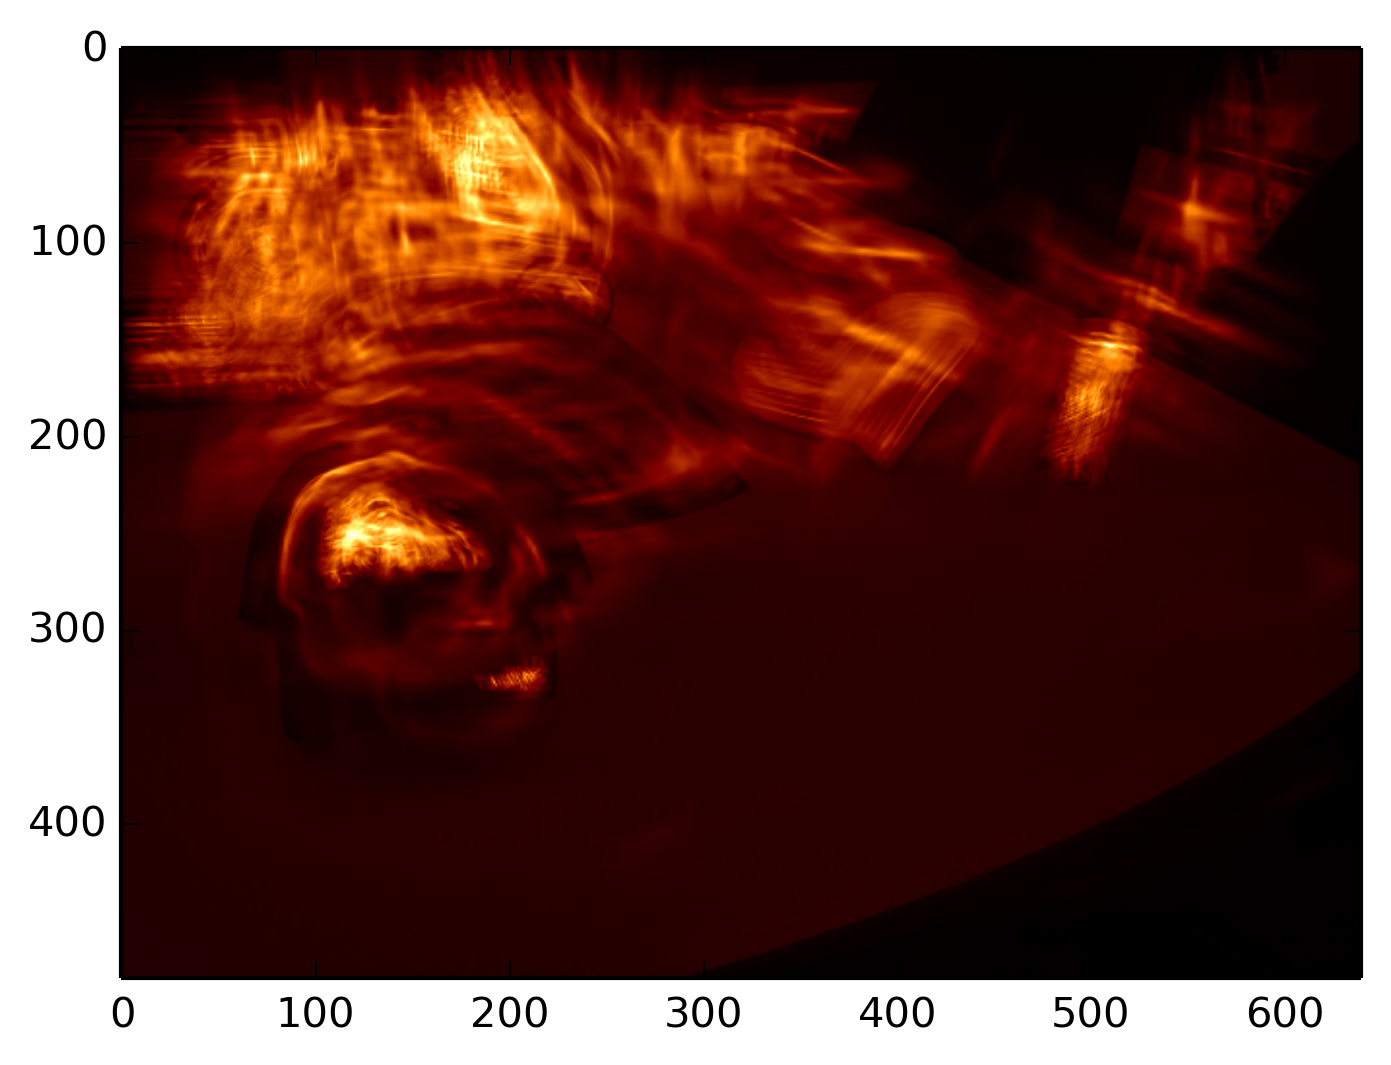
\includegraphics[width=\linewidth]{figures/meeting_smag_9}\end{subfigure}%
\begin{subfigure}[]{0.25\linewidth}\label{fig:meet_feats_4}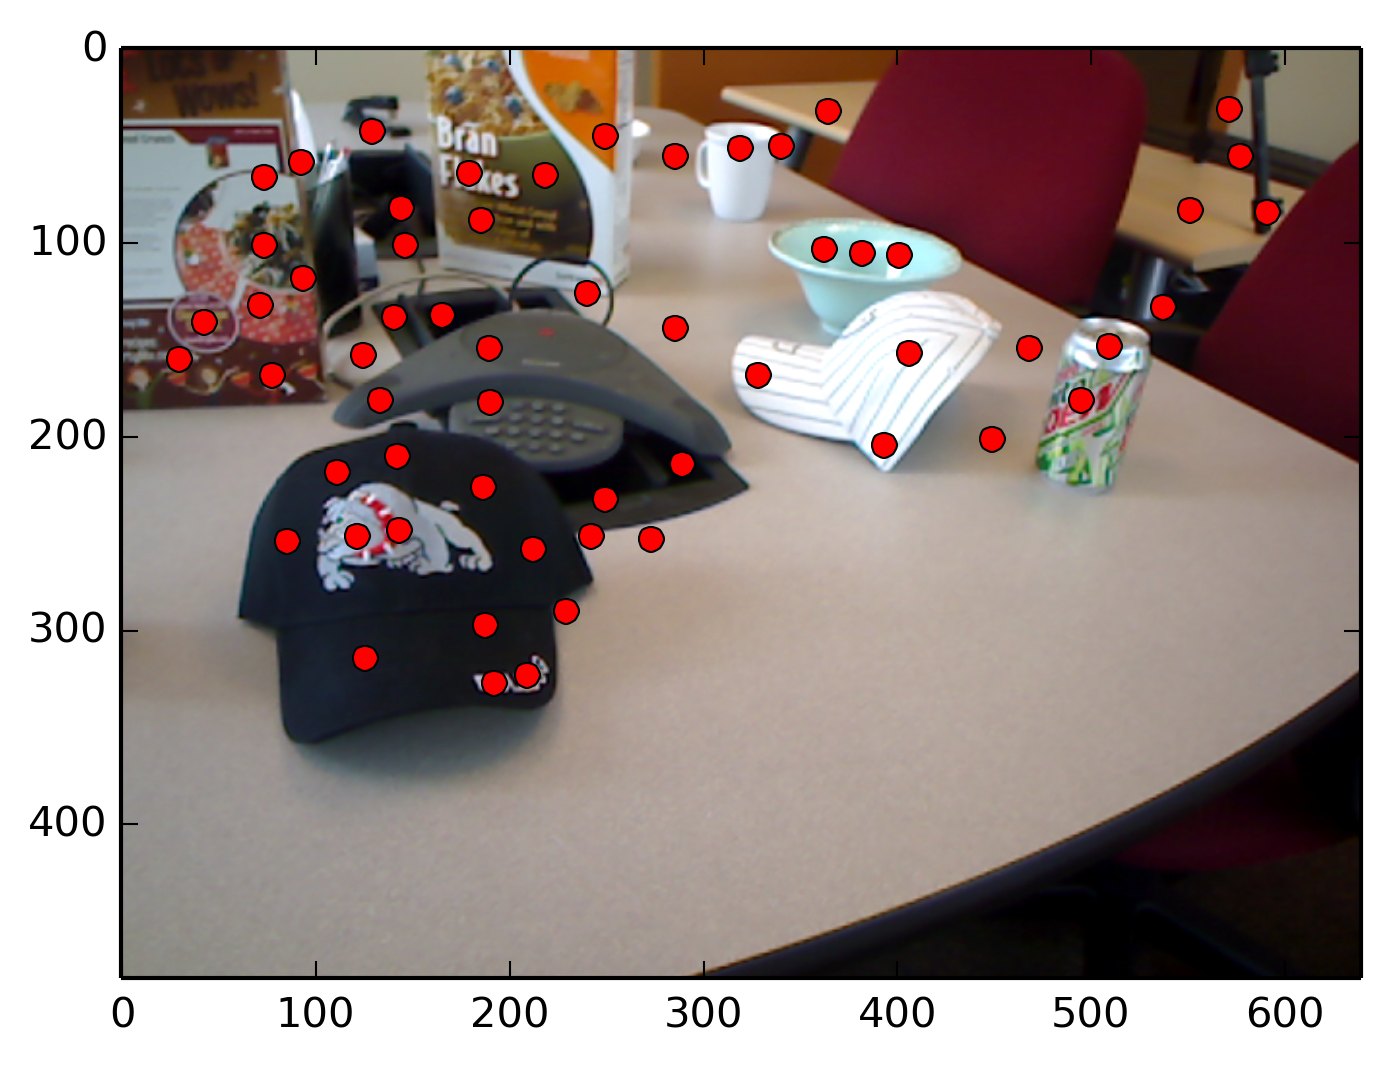
\includegraphics[width=\linewidth]{figures/meeting_feats_9}\end{subfigure}
\caption{Five consecutive images each of the \texttt{kitchen\_small} (left pair) and \texttt{meeting\_small} (right pair) scenes from the \texttt{rgbd\_scenes} dataset\cite{henry_rgb-d_2012}. For each pair, the computed symmetry magnitude is shown on the left, and the local maxima found using non-maximum suppression is shown on the left, using radius 15}
\label{fig:ex_xforms}
\end{figure}

The images show significant detection coverage in the image regions with objects, although there are keypoints found in ``stuff'' regions (\eg the front of the kitchen counter), and the keypoints are not stable across multiple frames. In particular, while points fall within the object boundaries, due to the appearance of the object and the camera viewpoint, some keypoints change position over time. Therefore, this methodology should not be used to extract precision keypoints for image matching, and any use for extracting descriptors or image regions for object recognition should be robust to at least small variations in the position of the region centroid.

\section{Future work}
\label{sec:future}

While Reisfeld and Kootstra's work (and therefore this work) focused on 2D appearance, and Potapova et al. focused on 3D point cloud symmetry, we believe the next best step is to consider some combination of the two approaches that exploits the capabilities of each modality. For example, by combining approaches, we may be able to detect posters on walls (an object without detectable depth) as well as remove the spurious appearance based detections on the kitchen counter by checking for plane membership over extended bounds. 

\section{Conclusion}
\label{sec:conclusion}

This work documents the initial steps in a research program to find an object saliency algorithm for use in a continuous object discovery and learning system. We reviewed the mathematical appraoch to the problem, described the computational approach, and created a parallel kernel suitable for acceleration on a \gls{gpu}. We show the the significant performance improvement through parallelization, and discuss the qualitative results from a simple keypoint detector. 

\arlbibliography{Symmetry}

\gotooddpage
\baresection{List of Symbols, Acronyms, and Abbreviations}
%\printacronyms[include-classes=abbrev]
\renewcommand{\glossarysection}[2][]{} % hide the title
\printglossary[type=\acronymtype]
%\printacronyms

%%%%%%%%%%%%%%%%%%%%%%%%%%%%%%%%%%%%%%%%%%%%%%%%%%%%%%%%%%%%%%%%%%%%%%%%%%%%%%%%
%% DISTRIBUTION LIST
\gotooddpage
\distlistsetup
\begin{distributionlist}
  \input{\MandatoryDL}
  \input{\UserDL}
\end{distributionlist}
\distlistcleanup
\finishonevenpage

\end{document}


%%% Local Variables: ***
%%% mode:latex ***
%%% reftex-default-bibliography: ("Symmetry.bib") ***
%%% End: ***
